\chapter{Tests and Analyses}
\label{sec:analysen}

This chapter evaluates the performance of the entire system. The assessment is based on AI-generated video data that was not presented to the system during the training phase. The focus is on the question of whether the improvements through temporal aggregation and the two-stage pipeline are more reliable than using object detection and segmentation alone. It is also of interest in which scenarios these additions have a clear influence on the system.


\section{Model Performance (Training \& Validation)}
Since the YOLO models have a significant influence on the reliability of the system, we first take a look at their isolated performance.

This section mainly addresses the training metrics. Of particular interest are the loss functions, which indicate how many errors occurred on the respective dataset (training or validation). The information from the confusion matrices provides insight into how many objects were detected, falsely detected or invented by the model.

\subsection{Performance of Object Detection}
The training metrics (Figure \ref{fig:training_det}) for the cat face detector show a continuously decreasing training loss and a high precision in validation over the course of 100 epochs.

\begin{figure}[H]
    \centering
    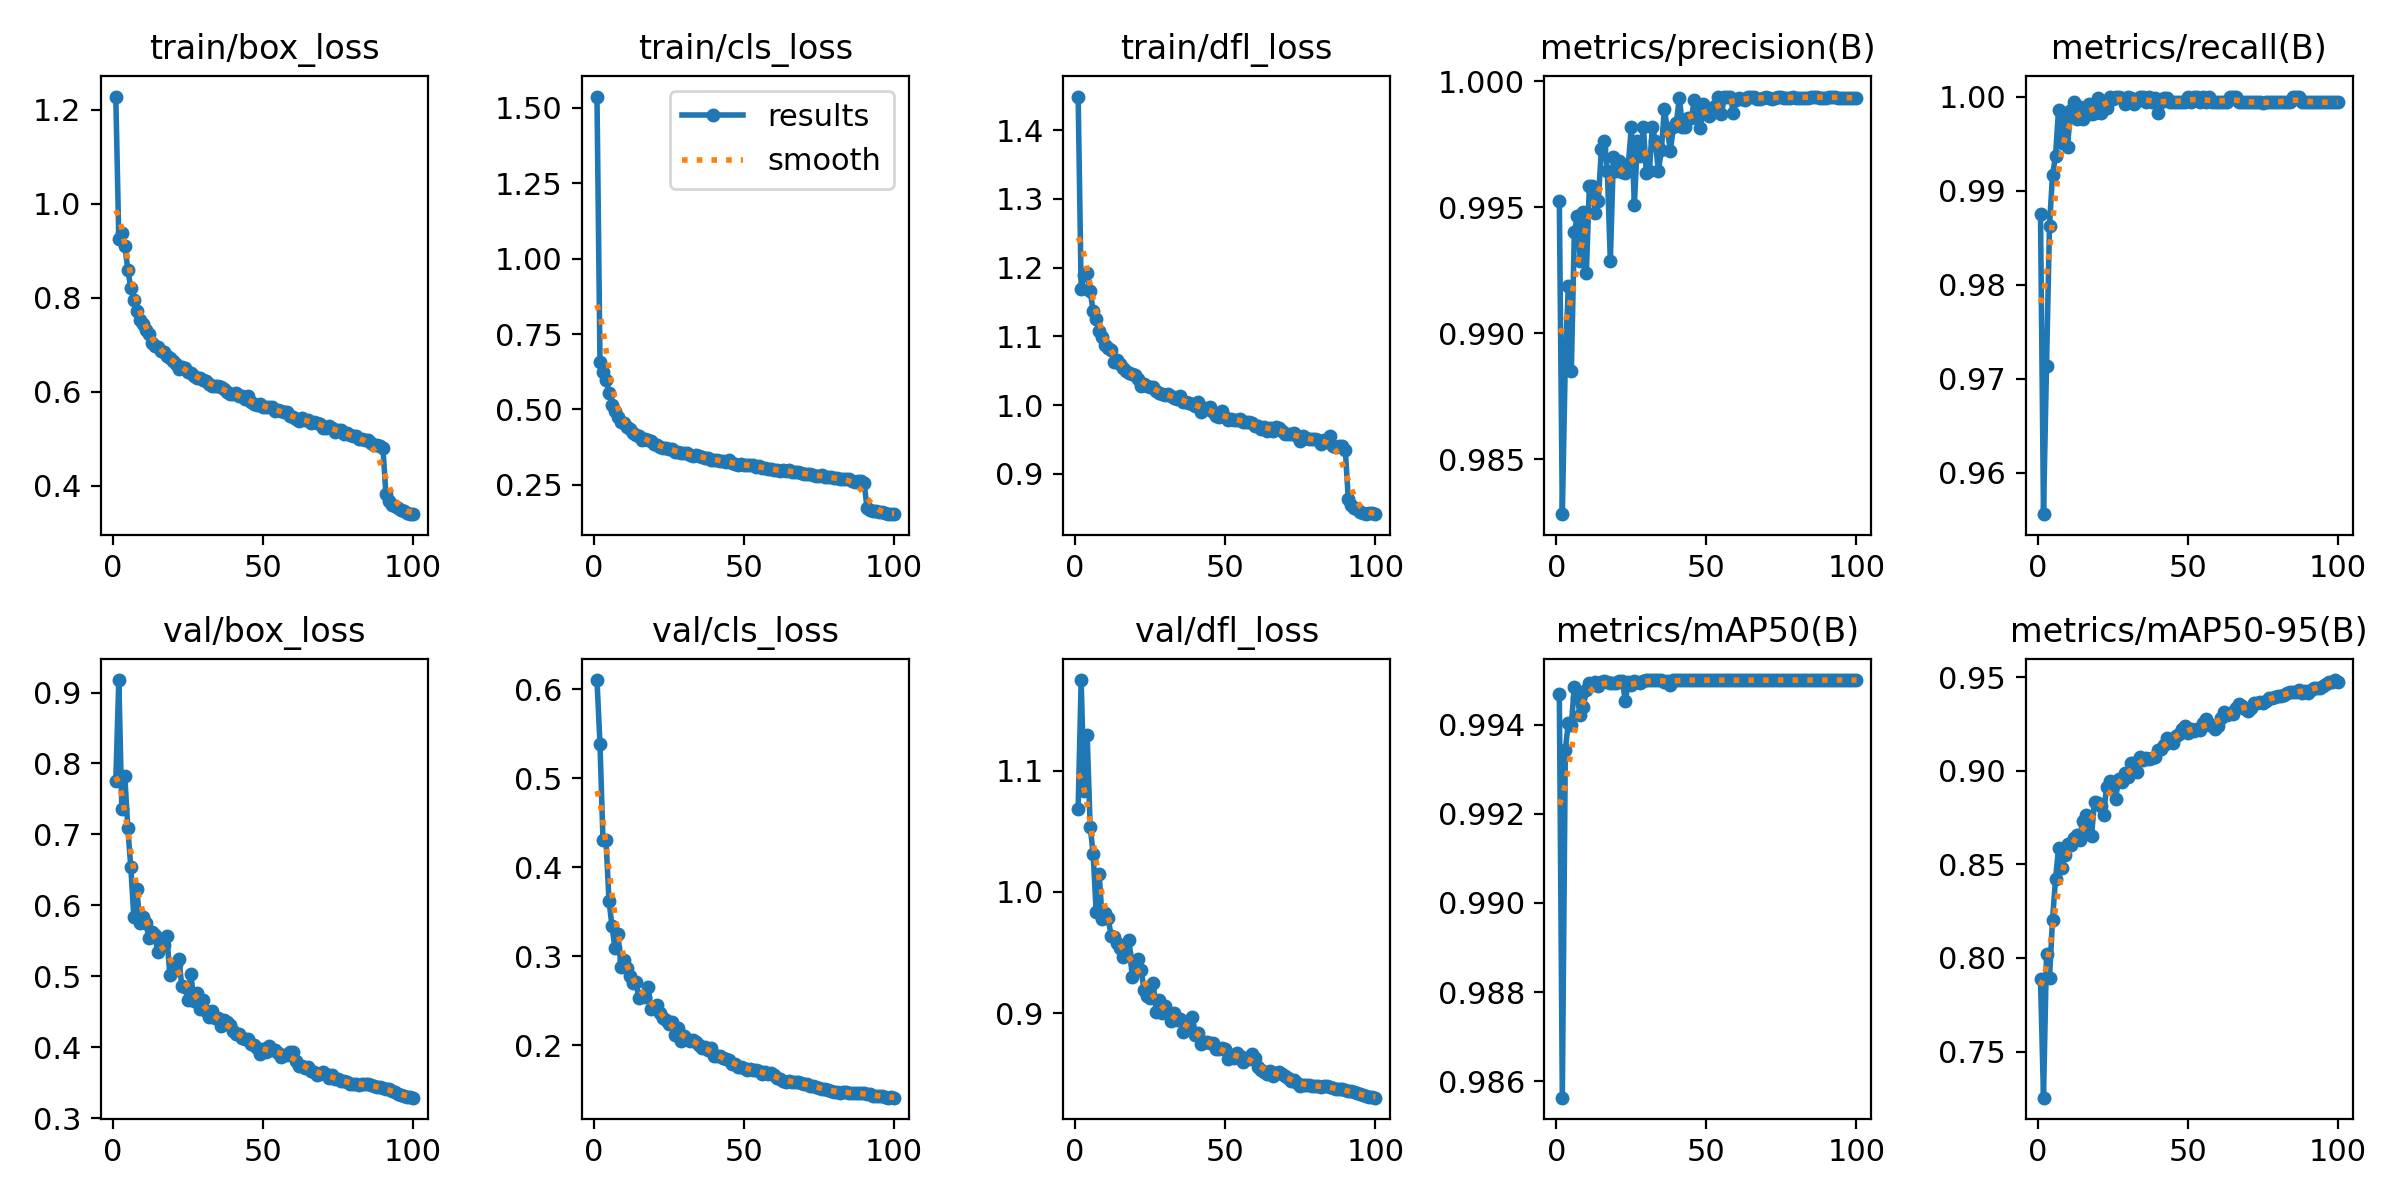
\includegraphics[width=0.8\textwidth]{images/results.png}
    \caption{Training progress and metrics of the YOLO object detector.}
    \label{fig:training_det}
\end{figure}

The confusion matrix of the object detection (Figure \ref{fig:confusion_det}) illustrates the precision of the localisation. It shows that 1,676 cat faces were correctly detected during validation. However, the model detected two cat faces where there was none, and it missed one completely. The matrix thus proves that the detector worked almost without errors on the validation data.

\begin{figure}[H]
    \centering
    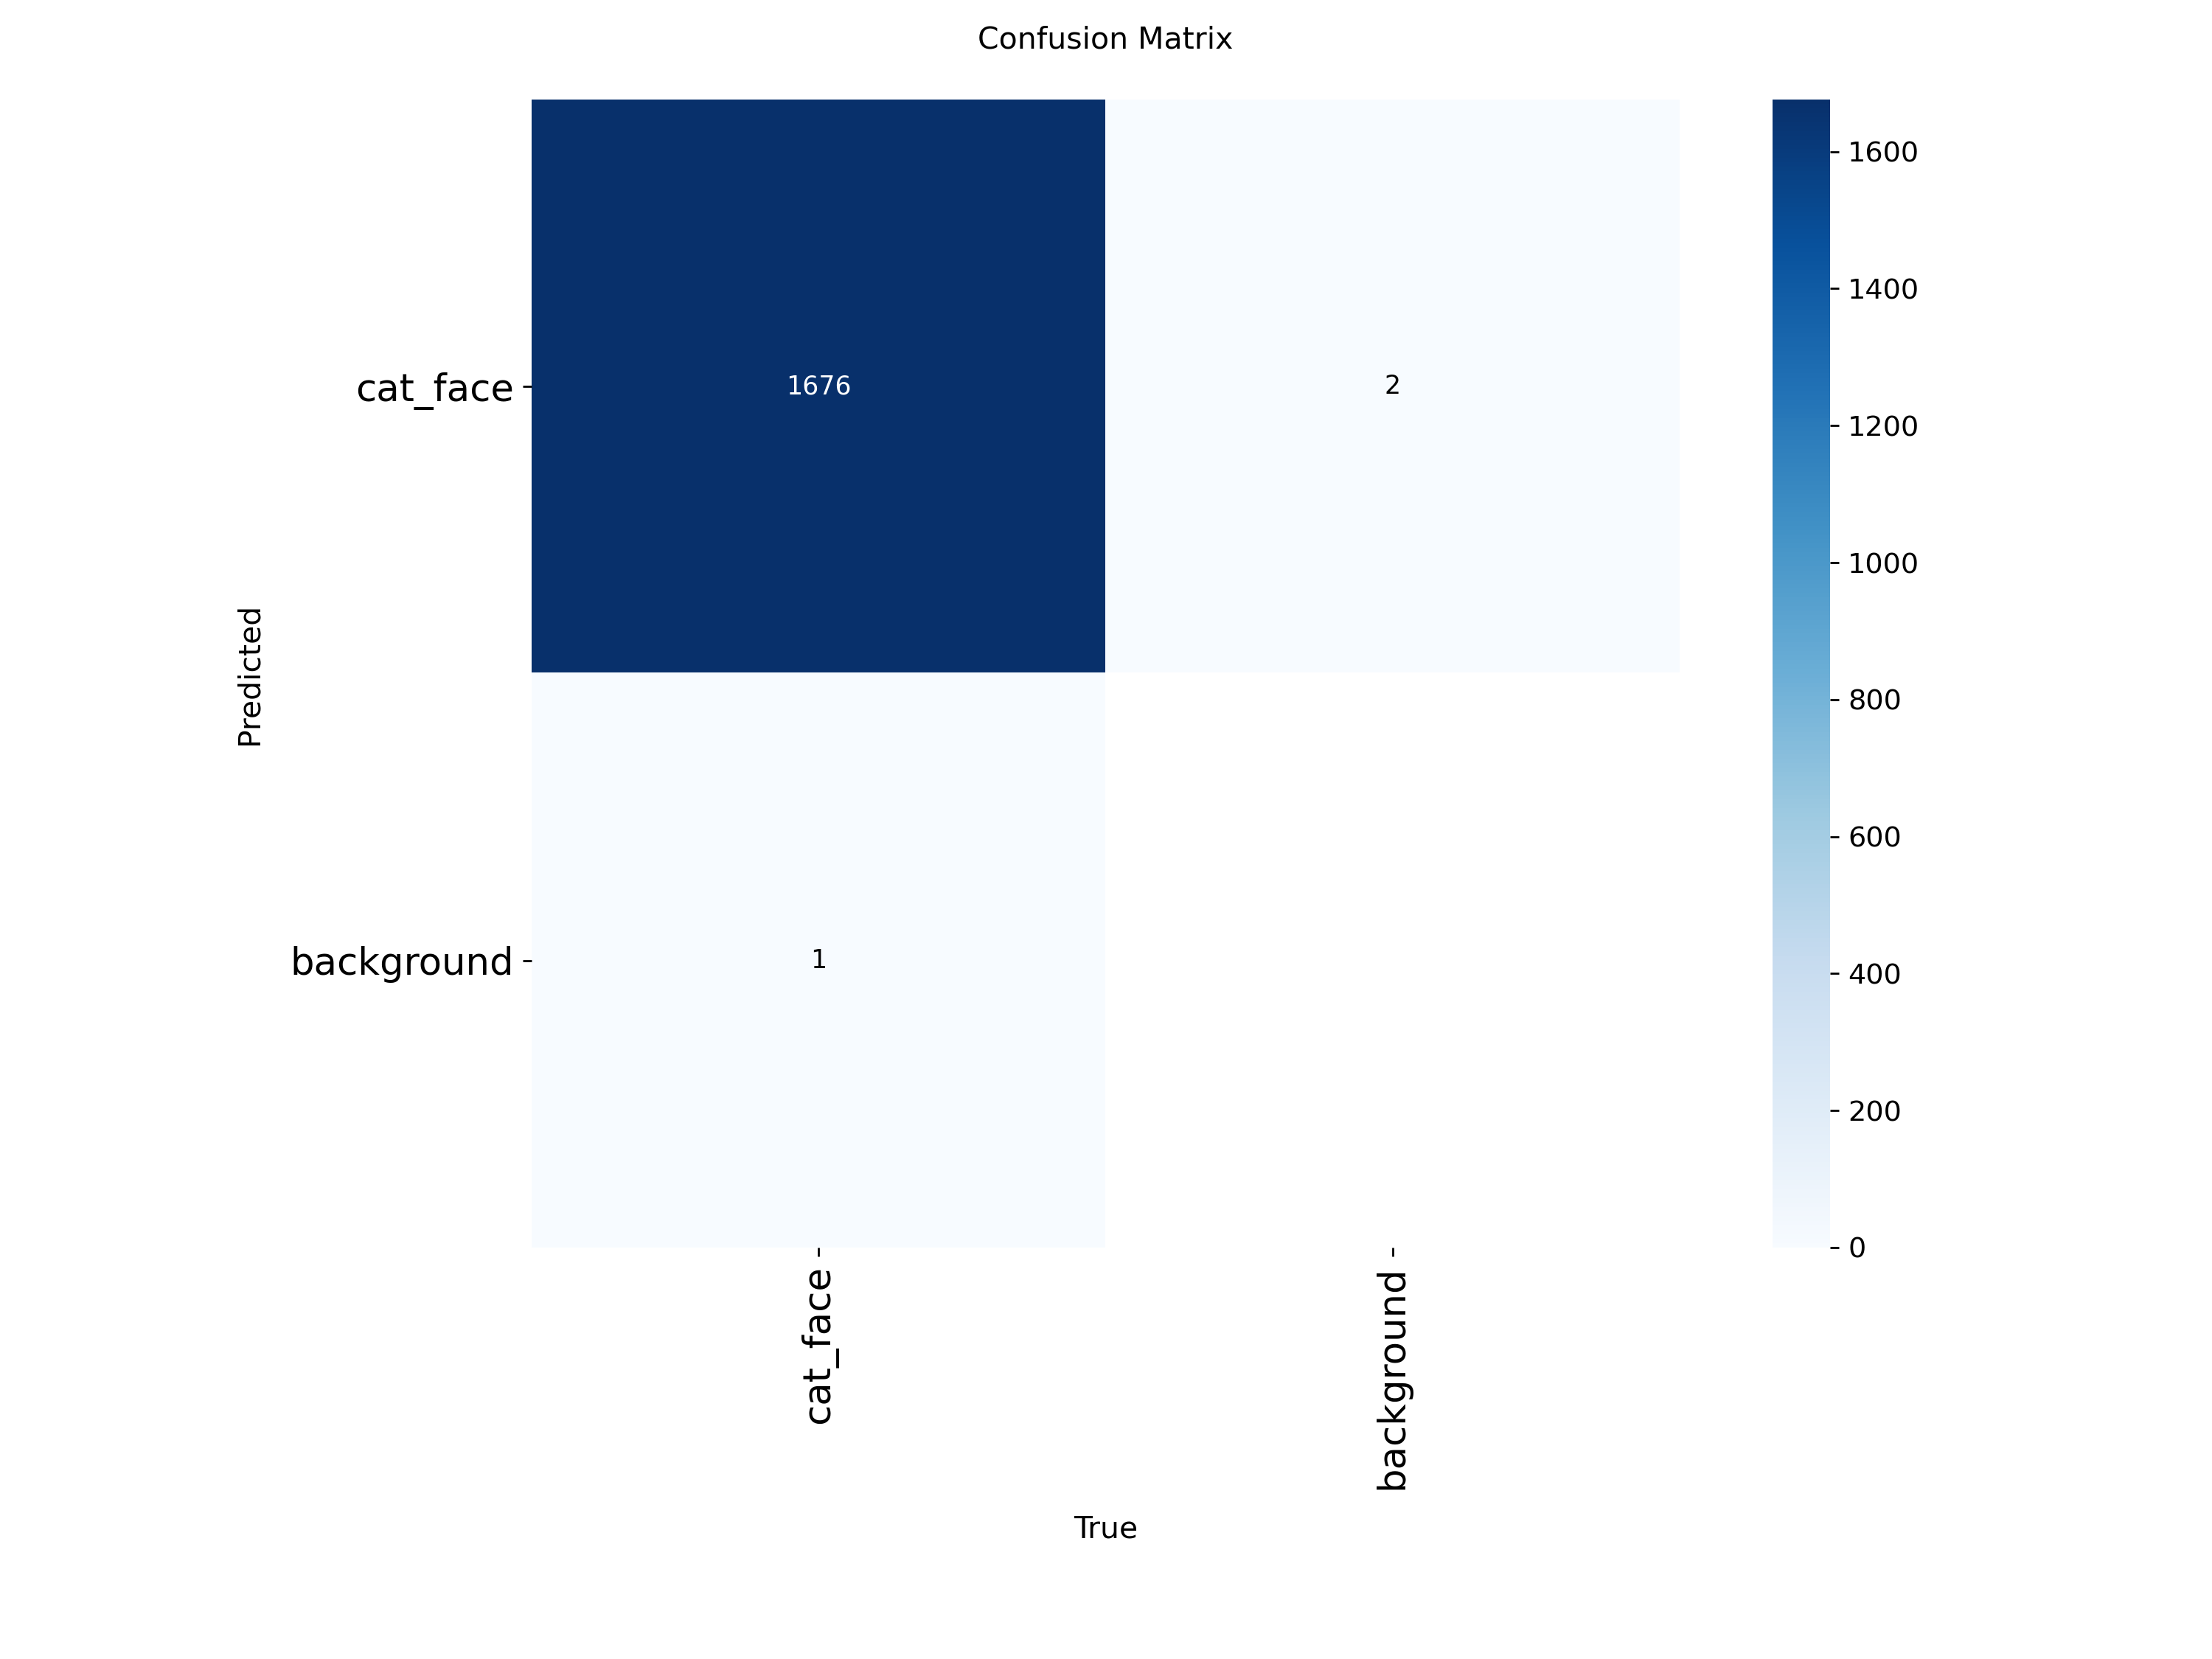
\includegraphics[width=0.6\textwidth]{images/confusion_matrix.png}
    \caption{Confusion matrix (detector).}
    \label{fig:confusion_det}
\end{figure}

An important metric, which is also based on the validation data, is the precision-recall curve; it indicates how confident the model is, through the ratio between correctly detected objects and false alarms \cite{everingham2010pascal, lin2014coco}. In this case, the curve shows that the model is extremely confident and does not have to guess when it sees a cat face.

\begin{figure}[H]
    \centering
    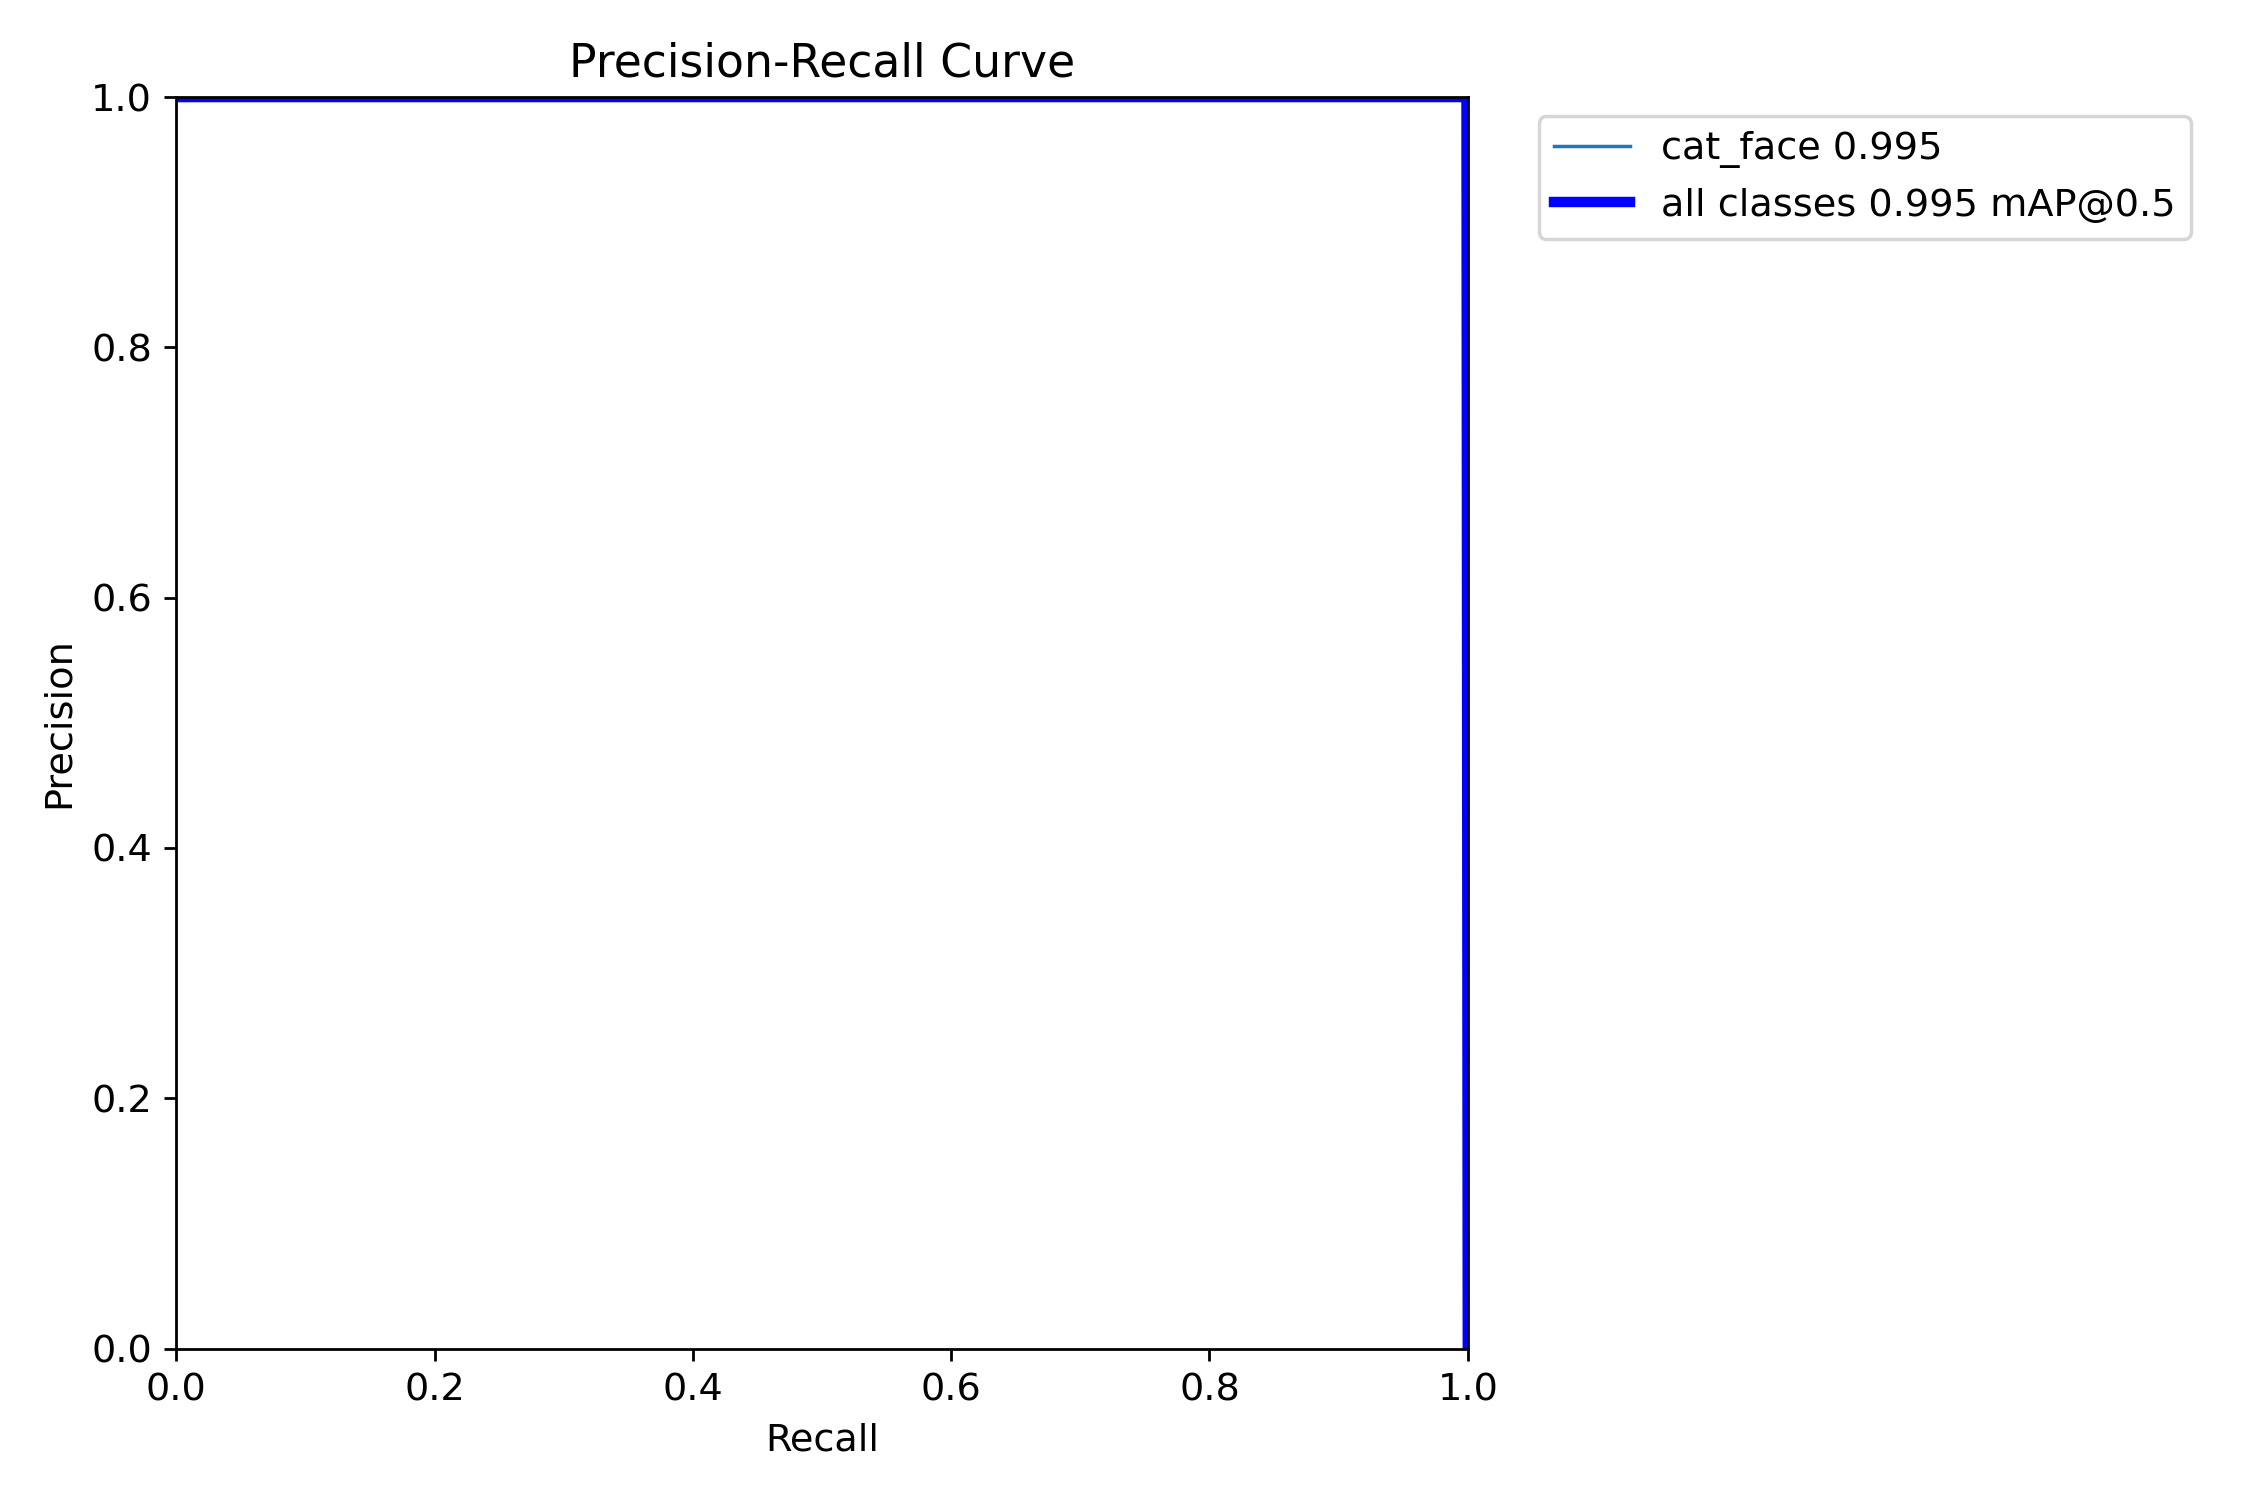
\includegraphics[width=0.6\textwidth]{images/BoxPR_curve.png}
    \caption{Precision-recall curve.}
    \label{fig:pr_curve_det}
\end{figure}

The F1 curve (Figure \ref{fig:f1_curve_det}) shows how the performance of the model changes when the confidence threshold \cite{ultralytics_confidence} is varied. This allows us to determine the optimal threshold for the real operation of the model. Since the curve stays flat up to $\approx 0.85$, i.e. no cat is missed here, it drops sharply above $0.85$. This shows that beyond this threshold, real cats are also easily missed. In practice, a confidence threshold of $\approx 0.75$ yields a good balance between ``cat is not detected'' and ``a cat is detected where there is none''. In operation, the detector is nevertheless run with a low threshold of 0.1, since ByteTrack also uses detections with a low confidence score for the association \cite{zhang2022bytetrack}.

\begin{figure}[H]
    \centering
    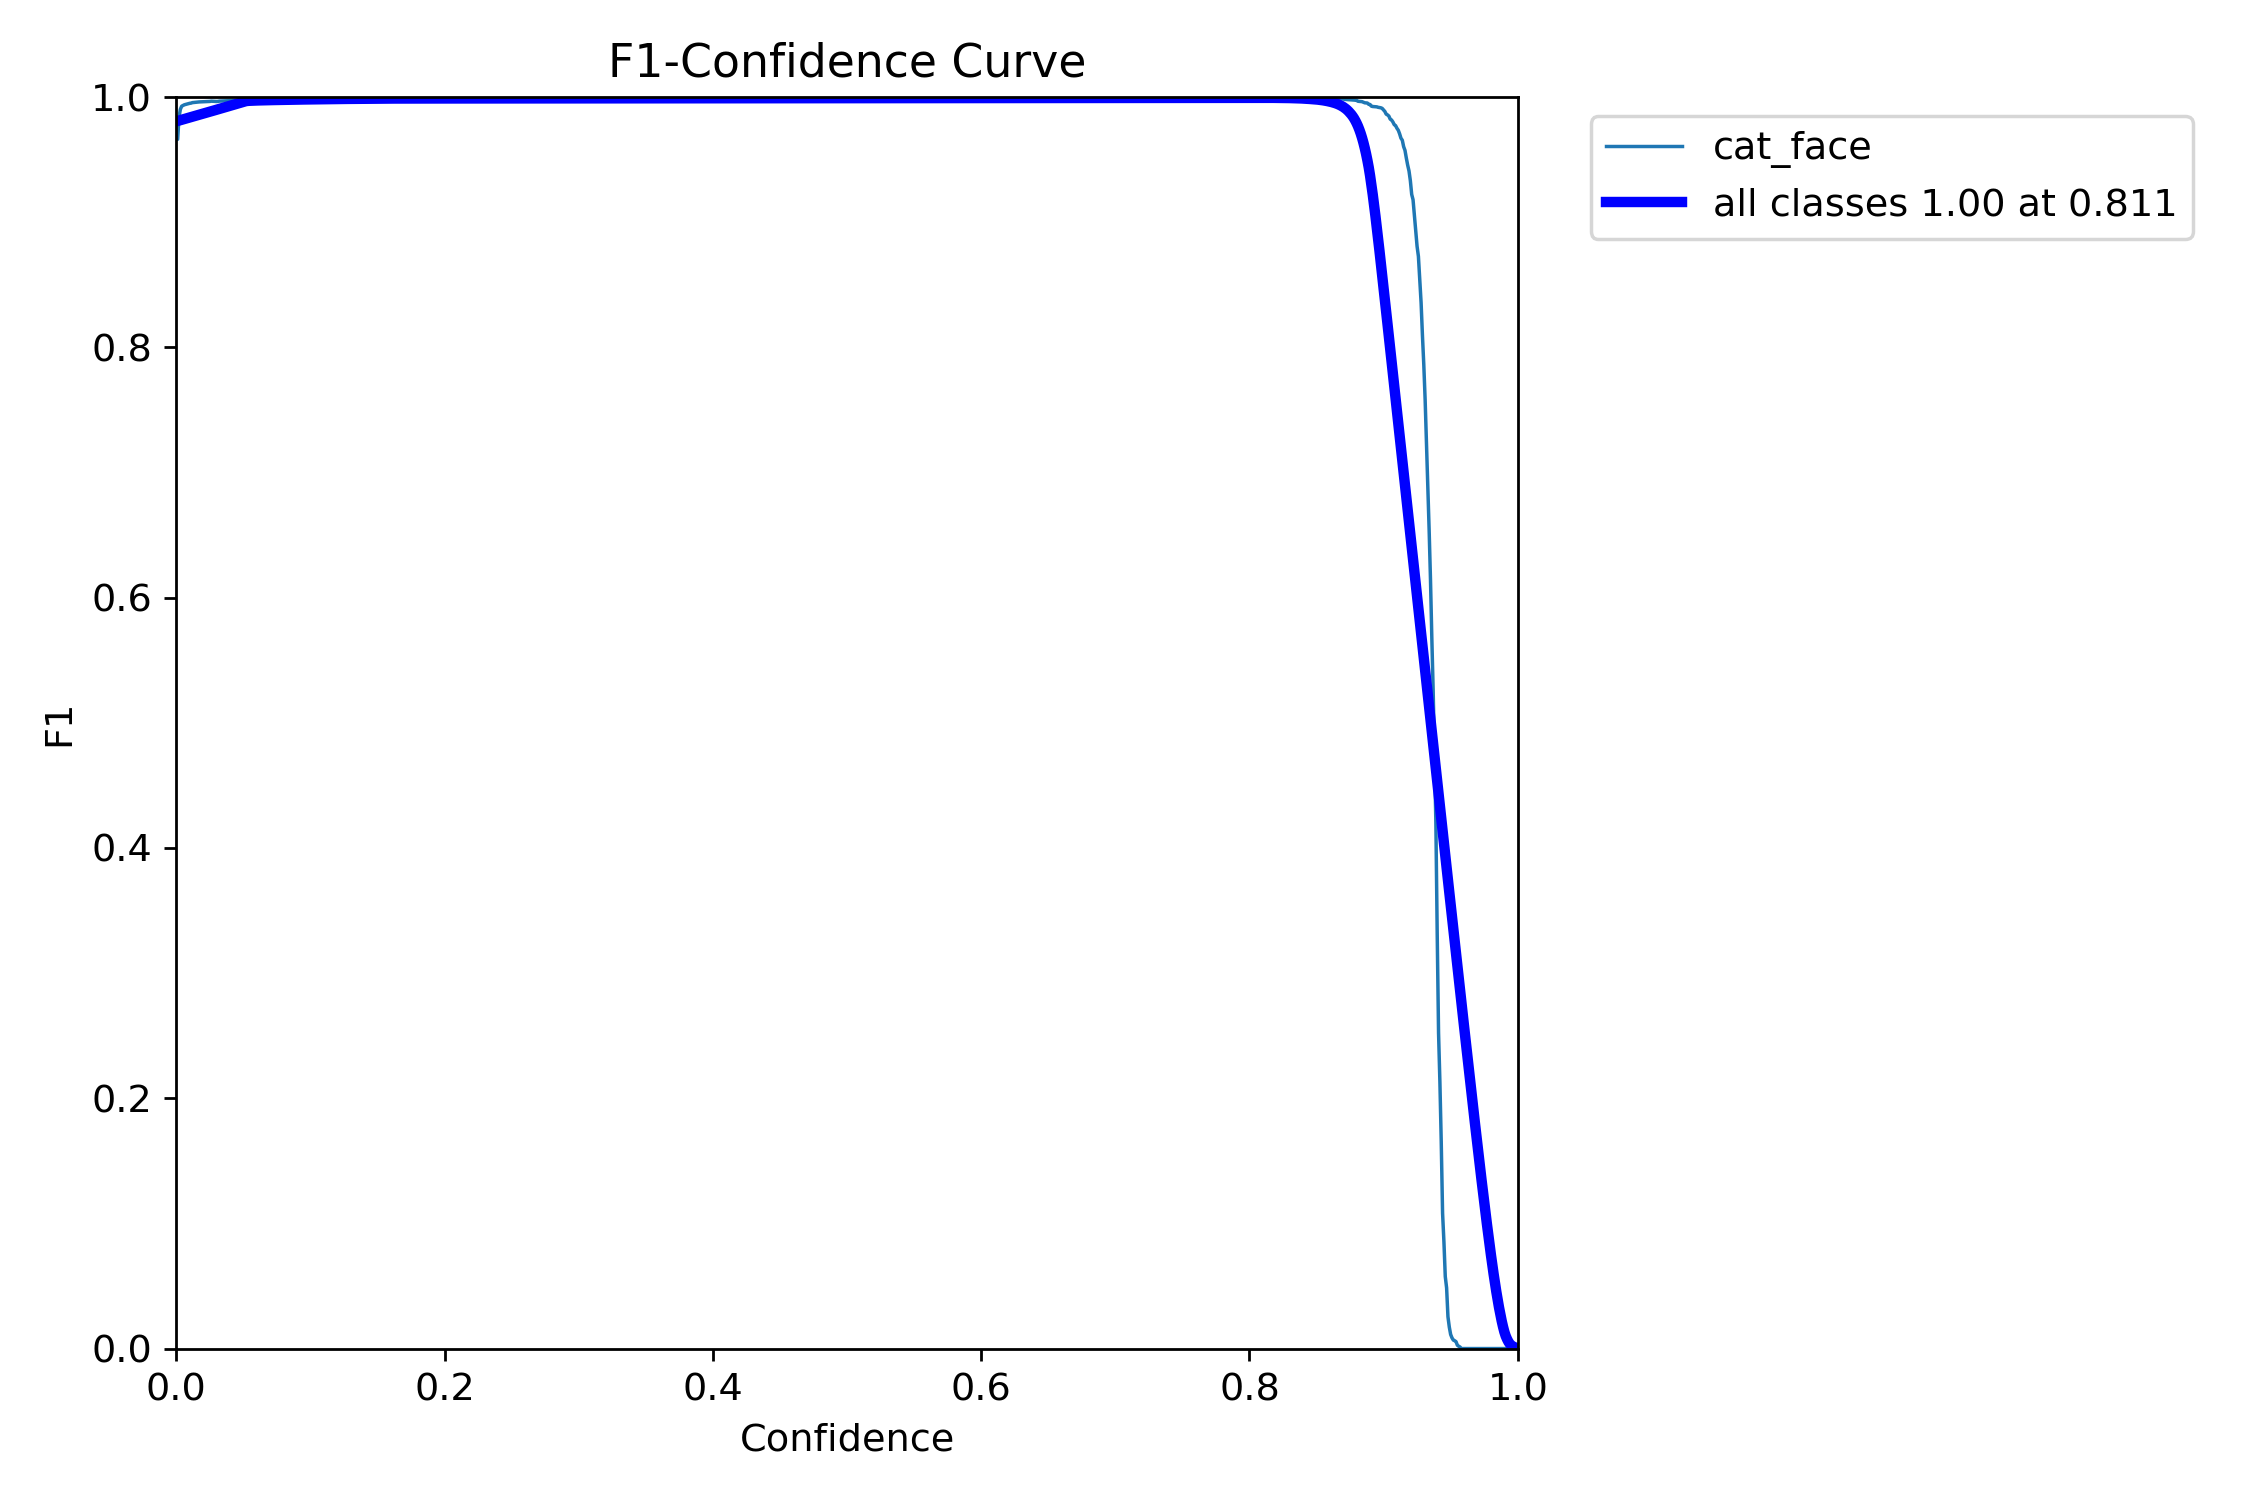
\includegraphics[width=0.6\textwidth]{images/BoxF1_curve.png}
    \caption{F1 curve.}
    \label{fig:f1_curve_det}
\end{figure}

Figure \ref{fig:val_pred_det} gives an impression of the detection performance of the model when it is applied to the validation data.

\begin{figure}[H]
    \centering
    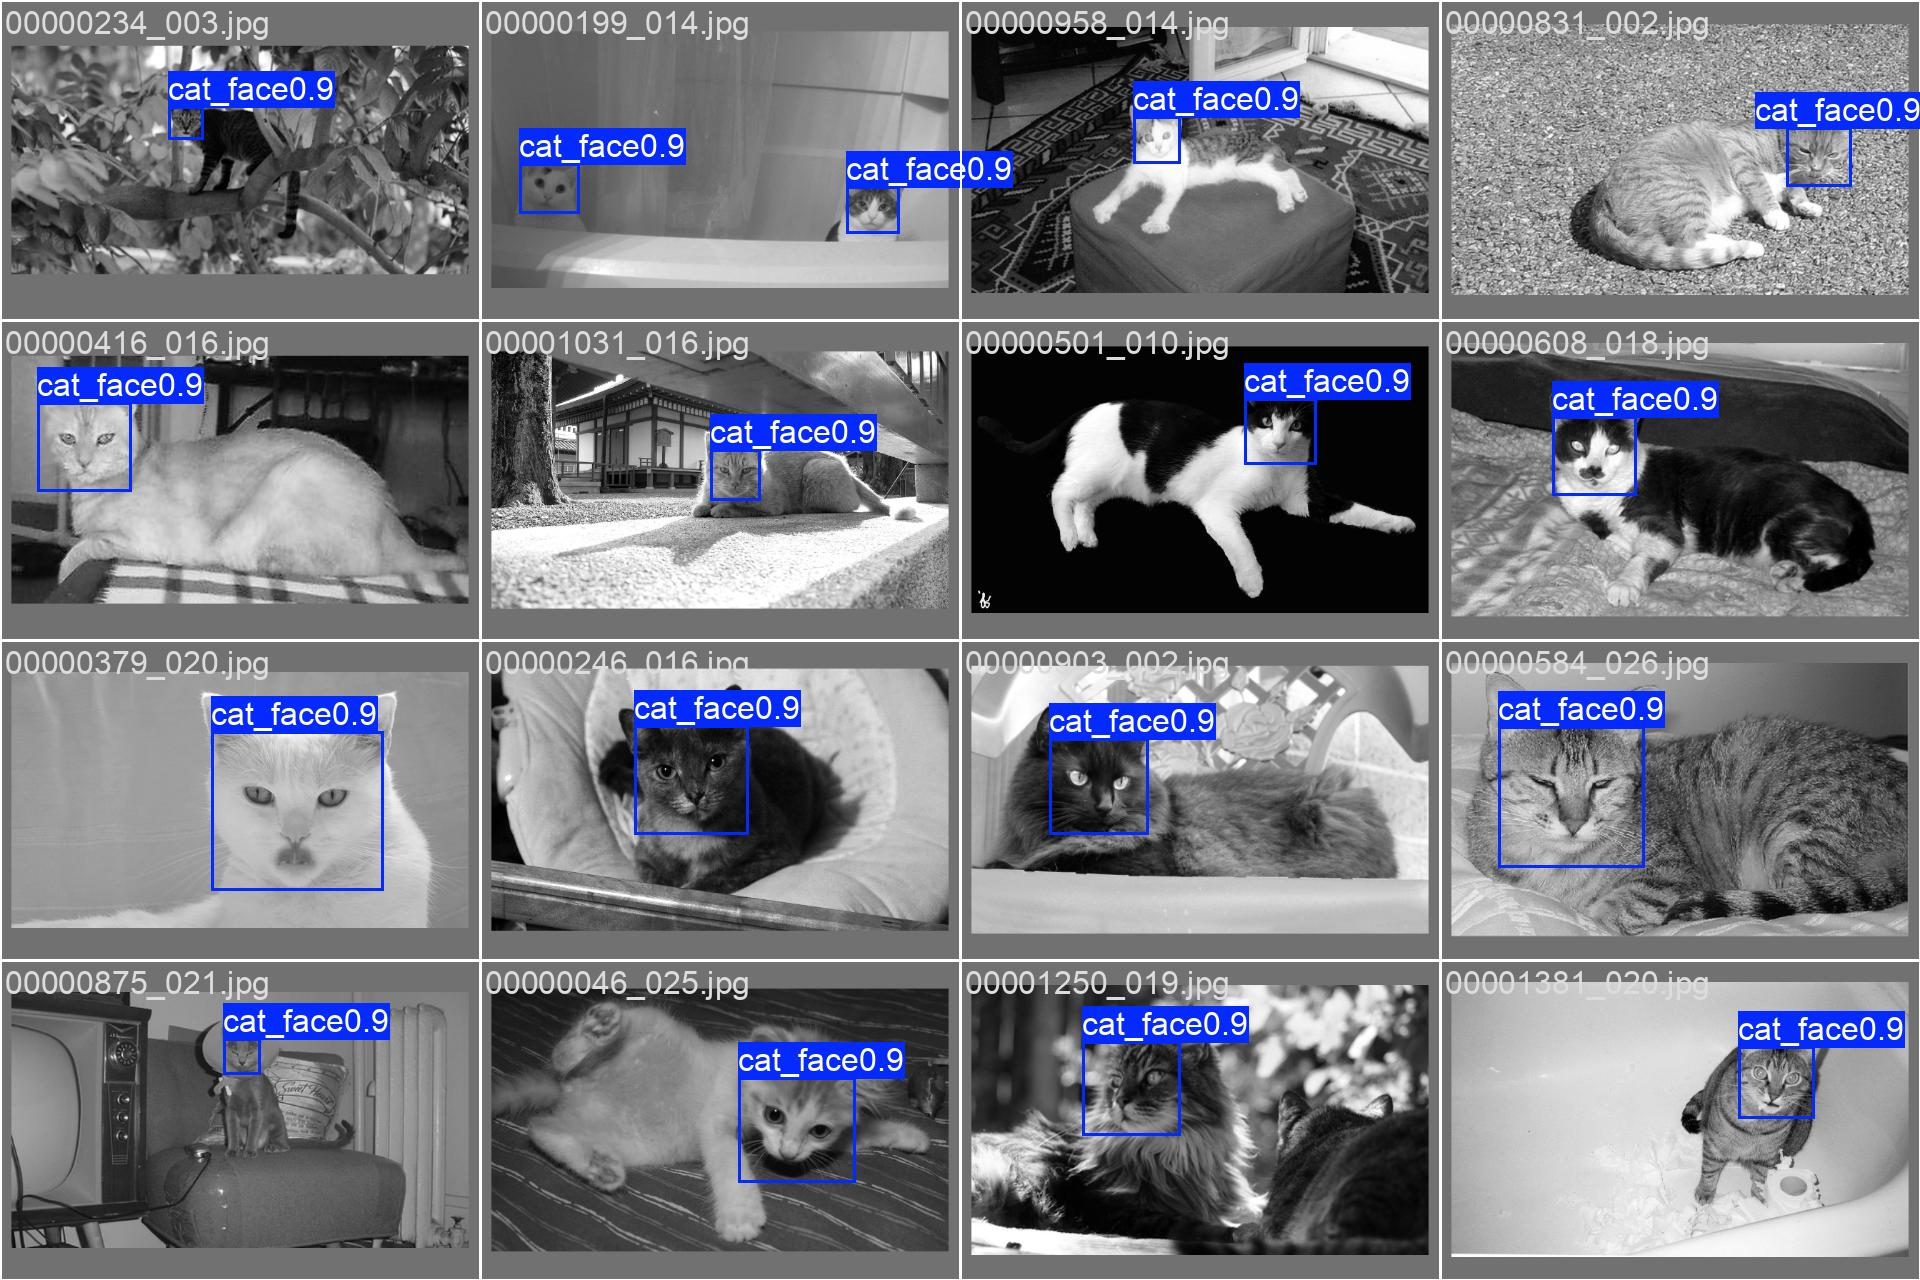
\includegraphics[width=0.8\textwidth]{images/val_batch0_pred.jpg}
    \caption{Predictions of the detector on the validation dataset.}
    \label{fig:val_pred_det}
\end{figure}

\subsection{Performance of Image Segmentation}
The following training metrics of the prey segmentation model show that the model has successfully learned its task.
Looking at the loss functions, it becomes apparent that the model makes fewer errors over the epochs in both training and validation; from this we can conclude that the segmentation model learns without overfitting too much to the training dataset.

\begin{figure}[H]
    \centering
    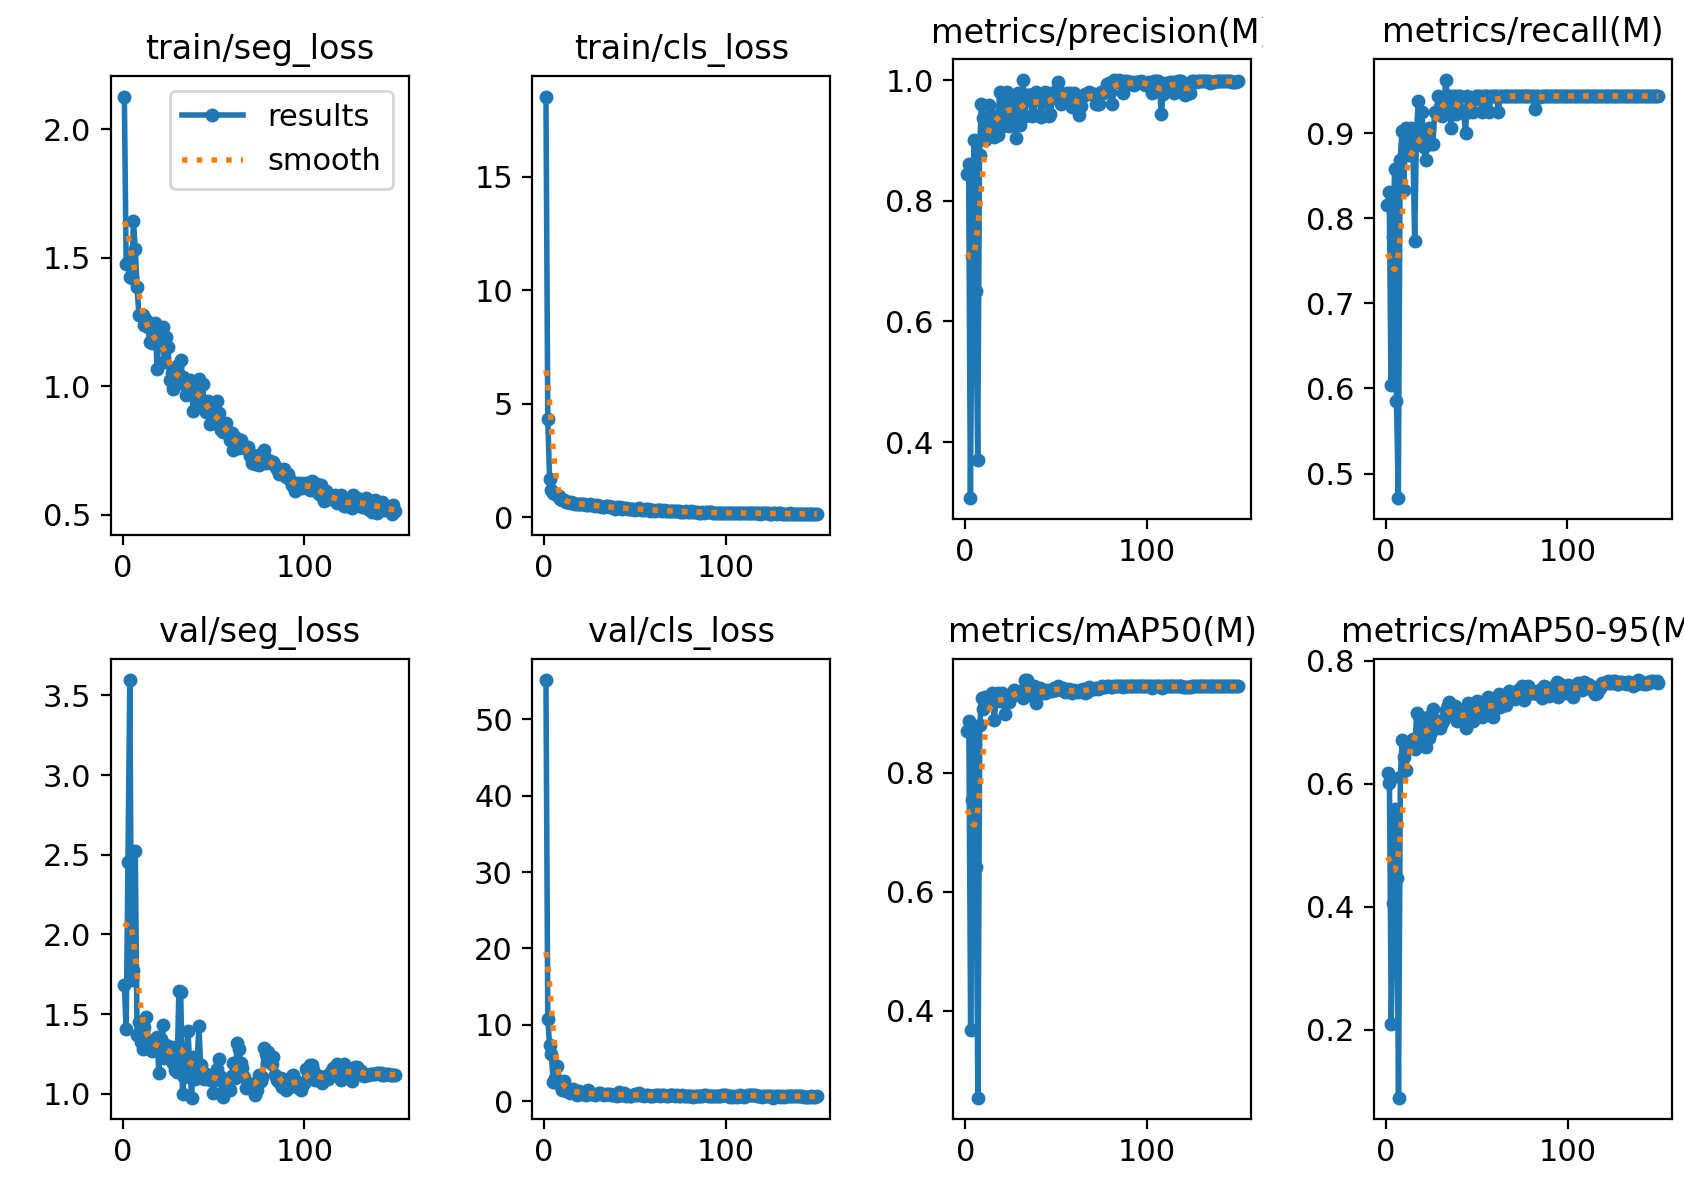
\includegraphics[width=0.8\textwidth]{images/seg_results.png}
    \caption{Training progress and metrics of the YOLO segmentation model.}
    \label{fig:training_cls}
\end{figure}

The precision-recall curve of the segmentation masks (Figure \ref{fig:pr_curve_seg}) shows that the model produces not a single false detection up to a recall of about 94\,\%. On the validation dataset, it achieves an mAP50 of 0.945.

\begin{figure}[H]
    \centering
    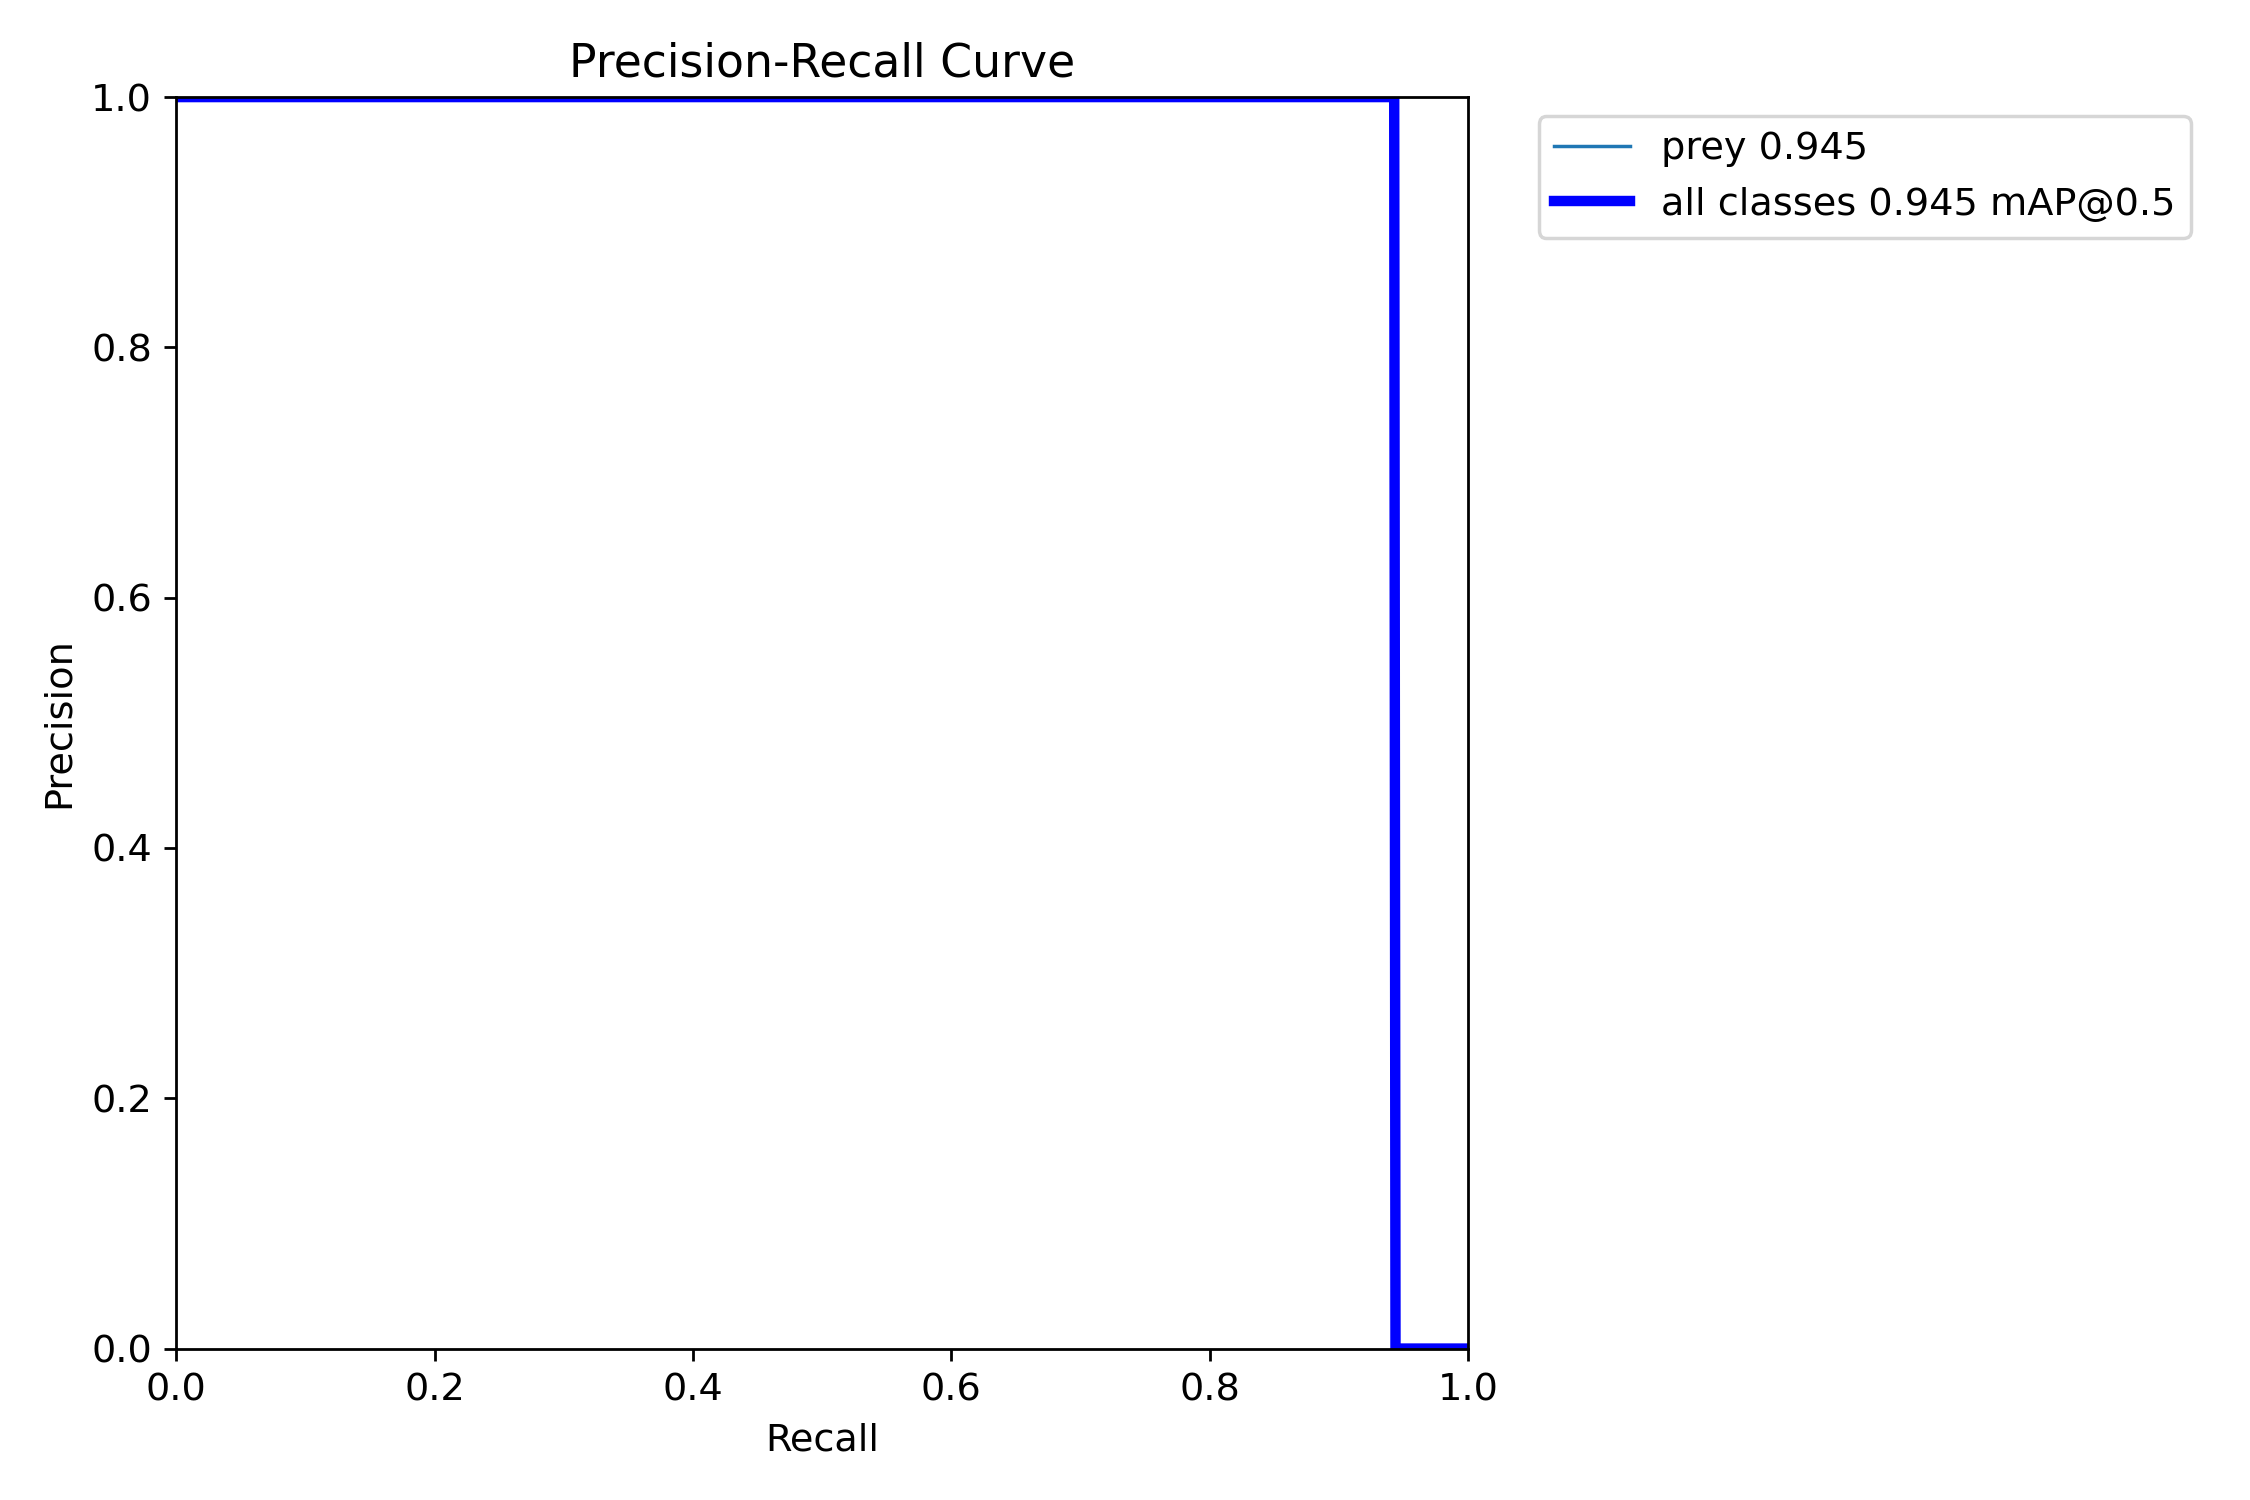
\includegraphics[width=0.6\textwidth]{images/seg_pr_curve.png}
    \caption{Precision-recall curve of the segmentation masks.}
    \label{fig:pr_curve_seg}
\end{figure}

The F1 curve (Figure \ref{fig:f1_curve_seg}) reaches its maximum of 0.97 at a confidence threshold of 0.728. Between about 0.1 and 0.85 it remains nearly constant, so in this range the model is hardly sensitive to the choice of threshold.

\begin{figure}[H]
    \centering
    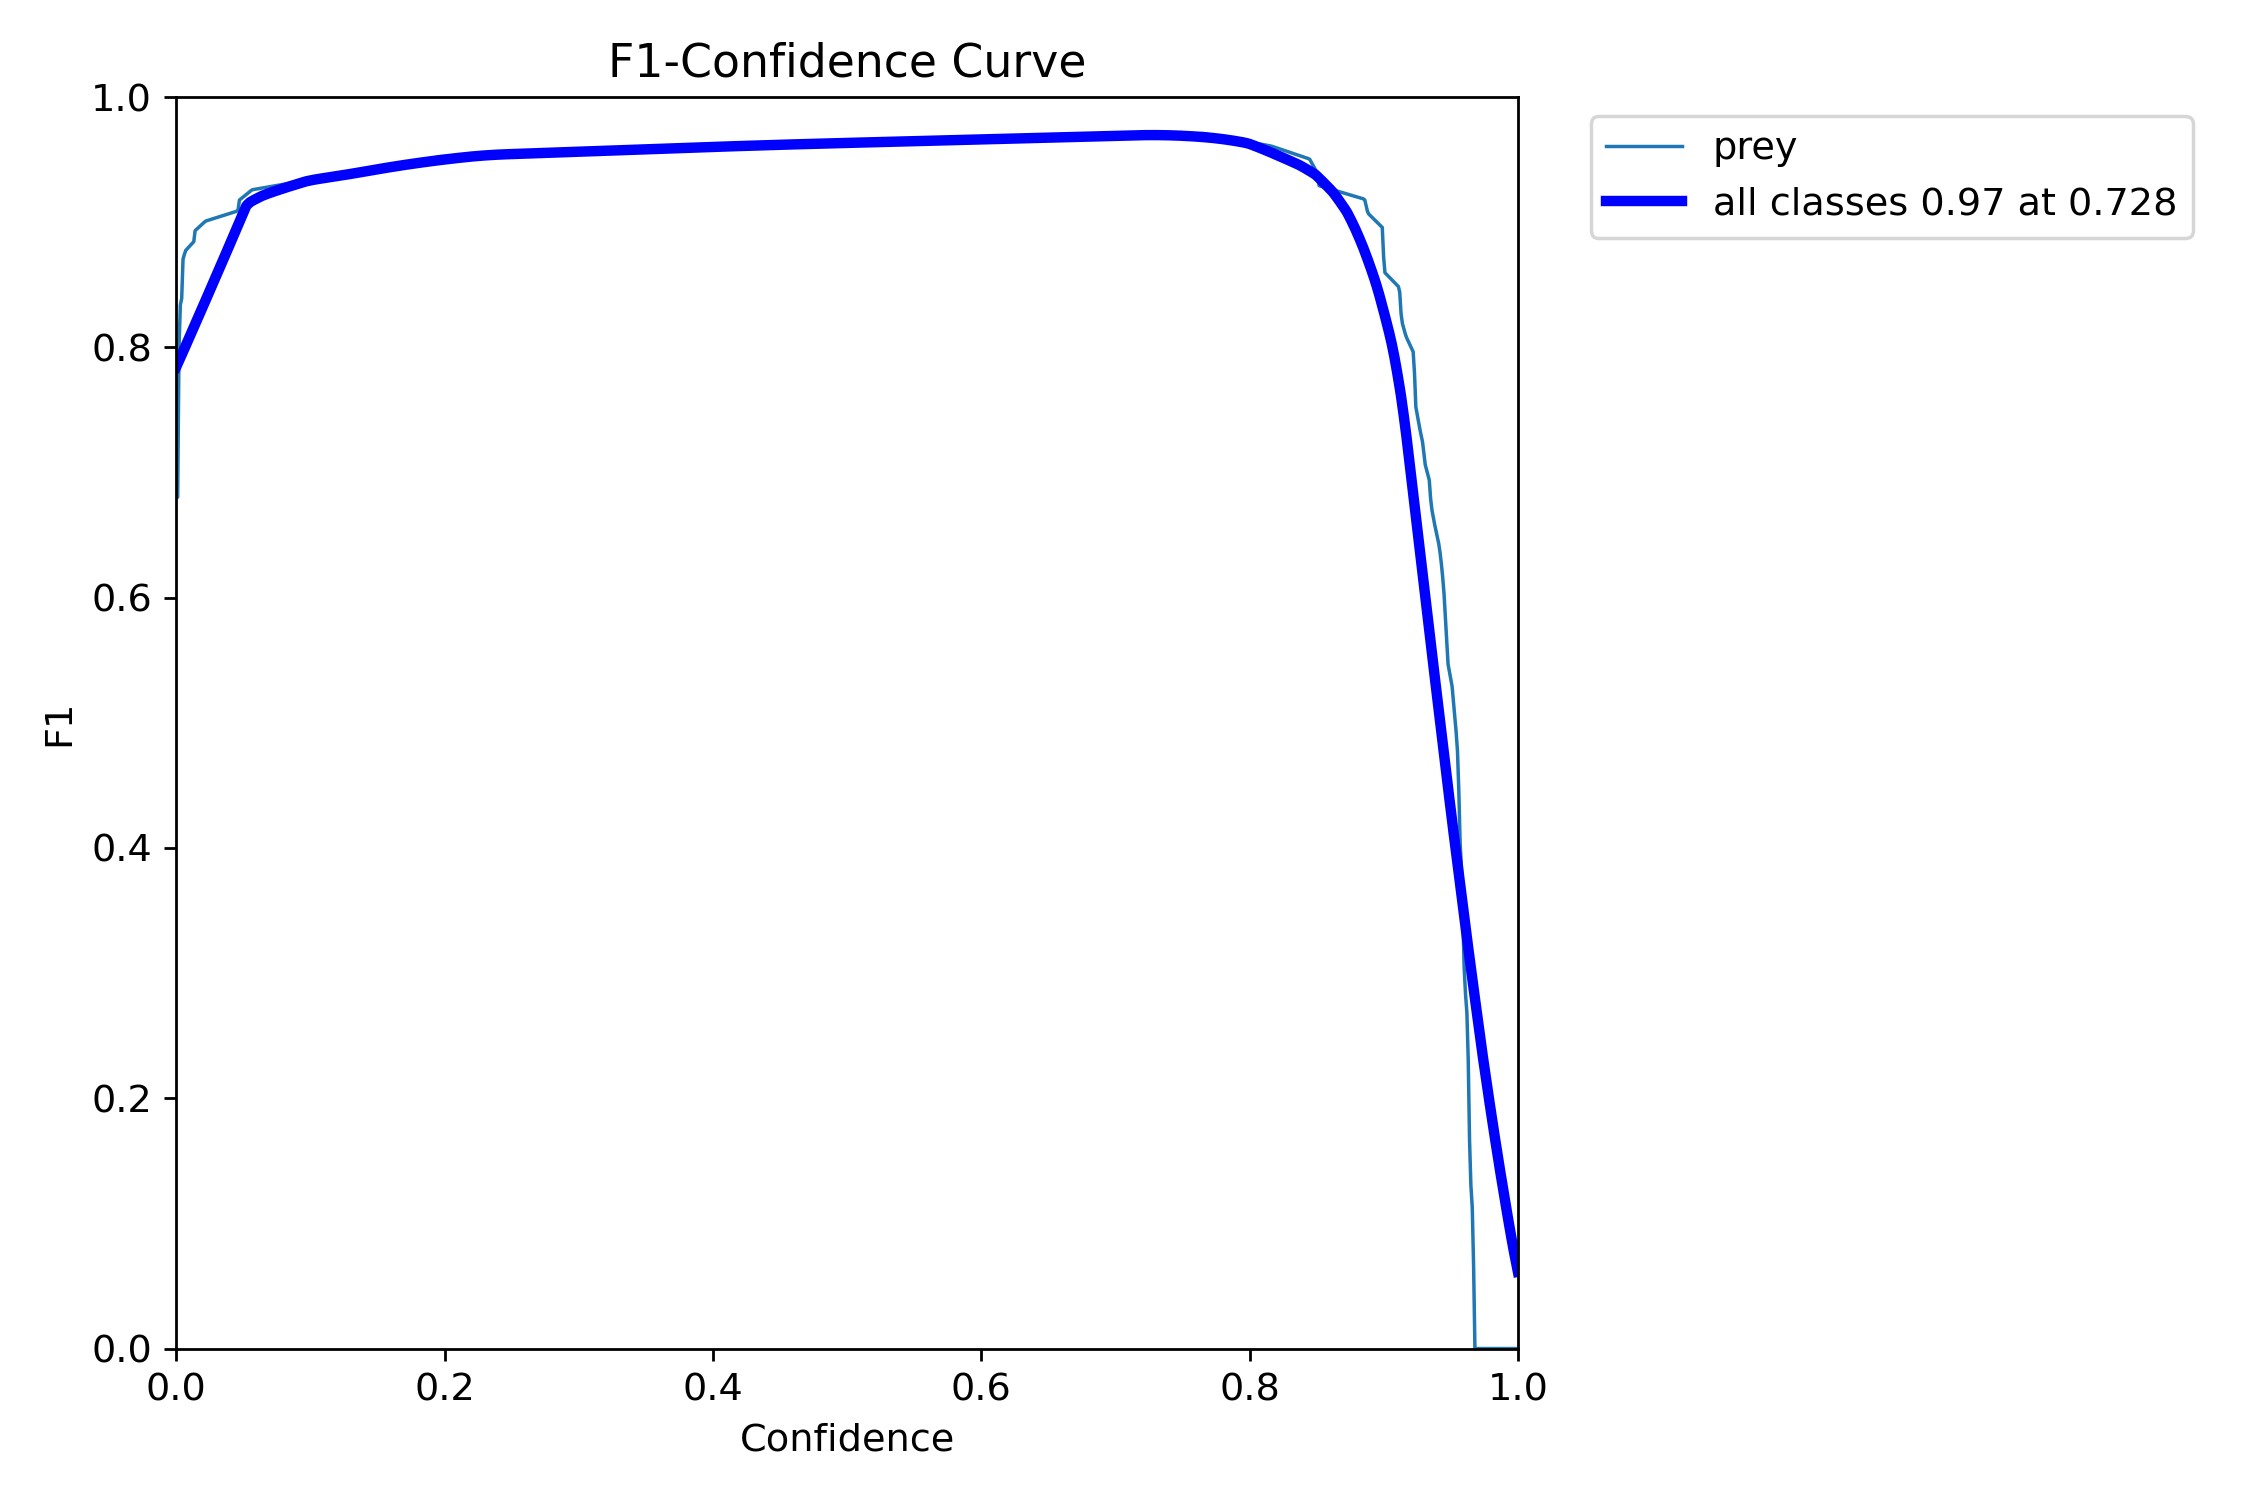
\includegraphics[width=0.6\textwidth]{images/seg_f1_curve.png}
    \caption{F1 curve of the segmentation model.}
    \label{fig:f1_curve_seg}
\end{figure}

Figure \ref{fig:val_pred_cls} makes it easy to see how well the model handles unknown data.

\begin{figure}[H]
    \centering
    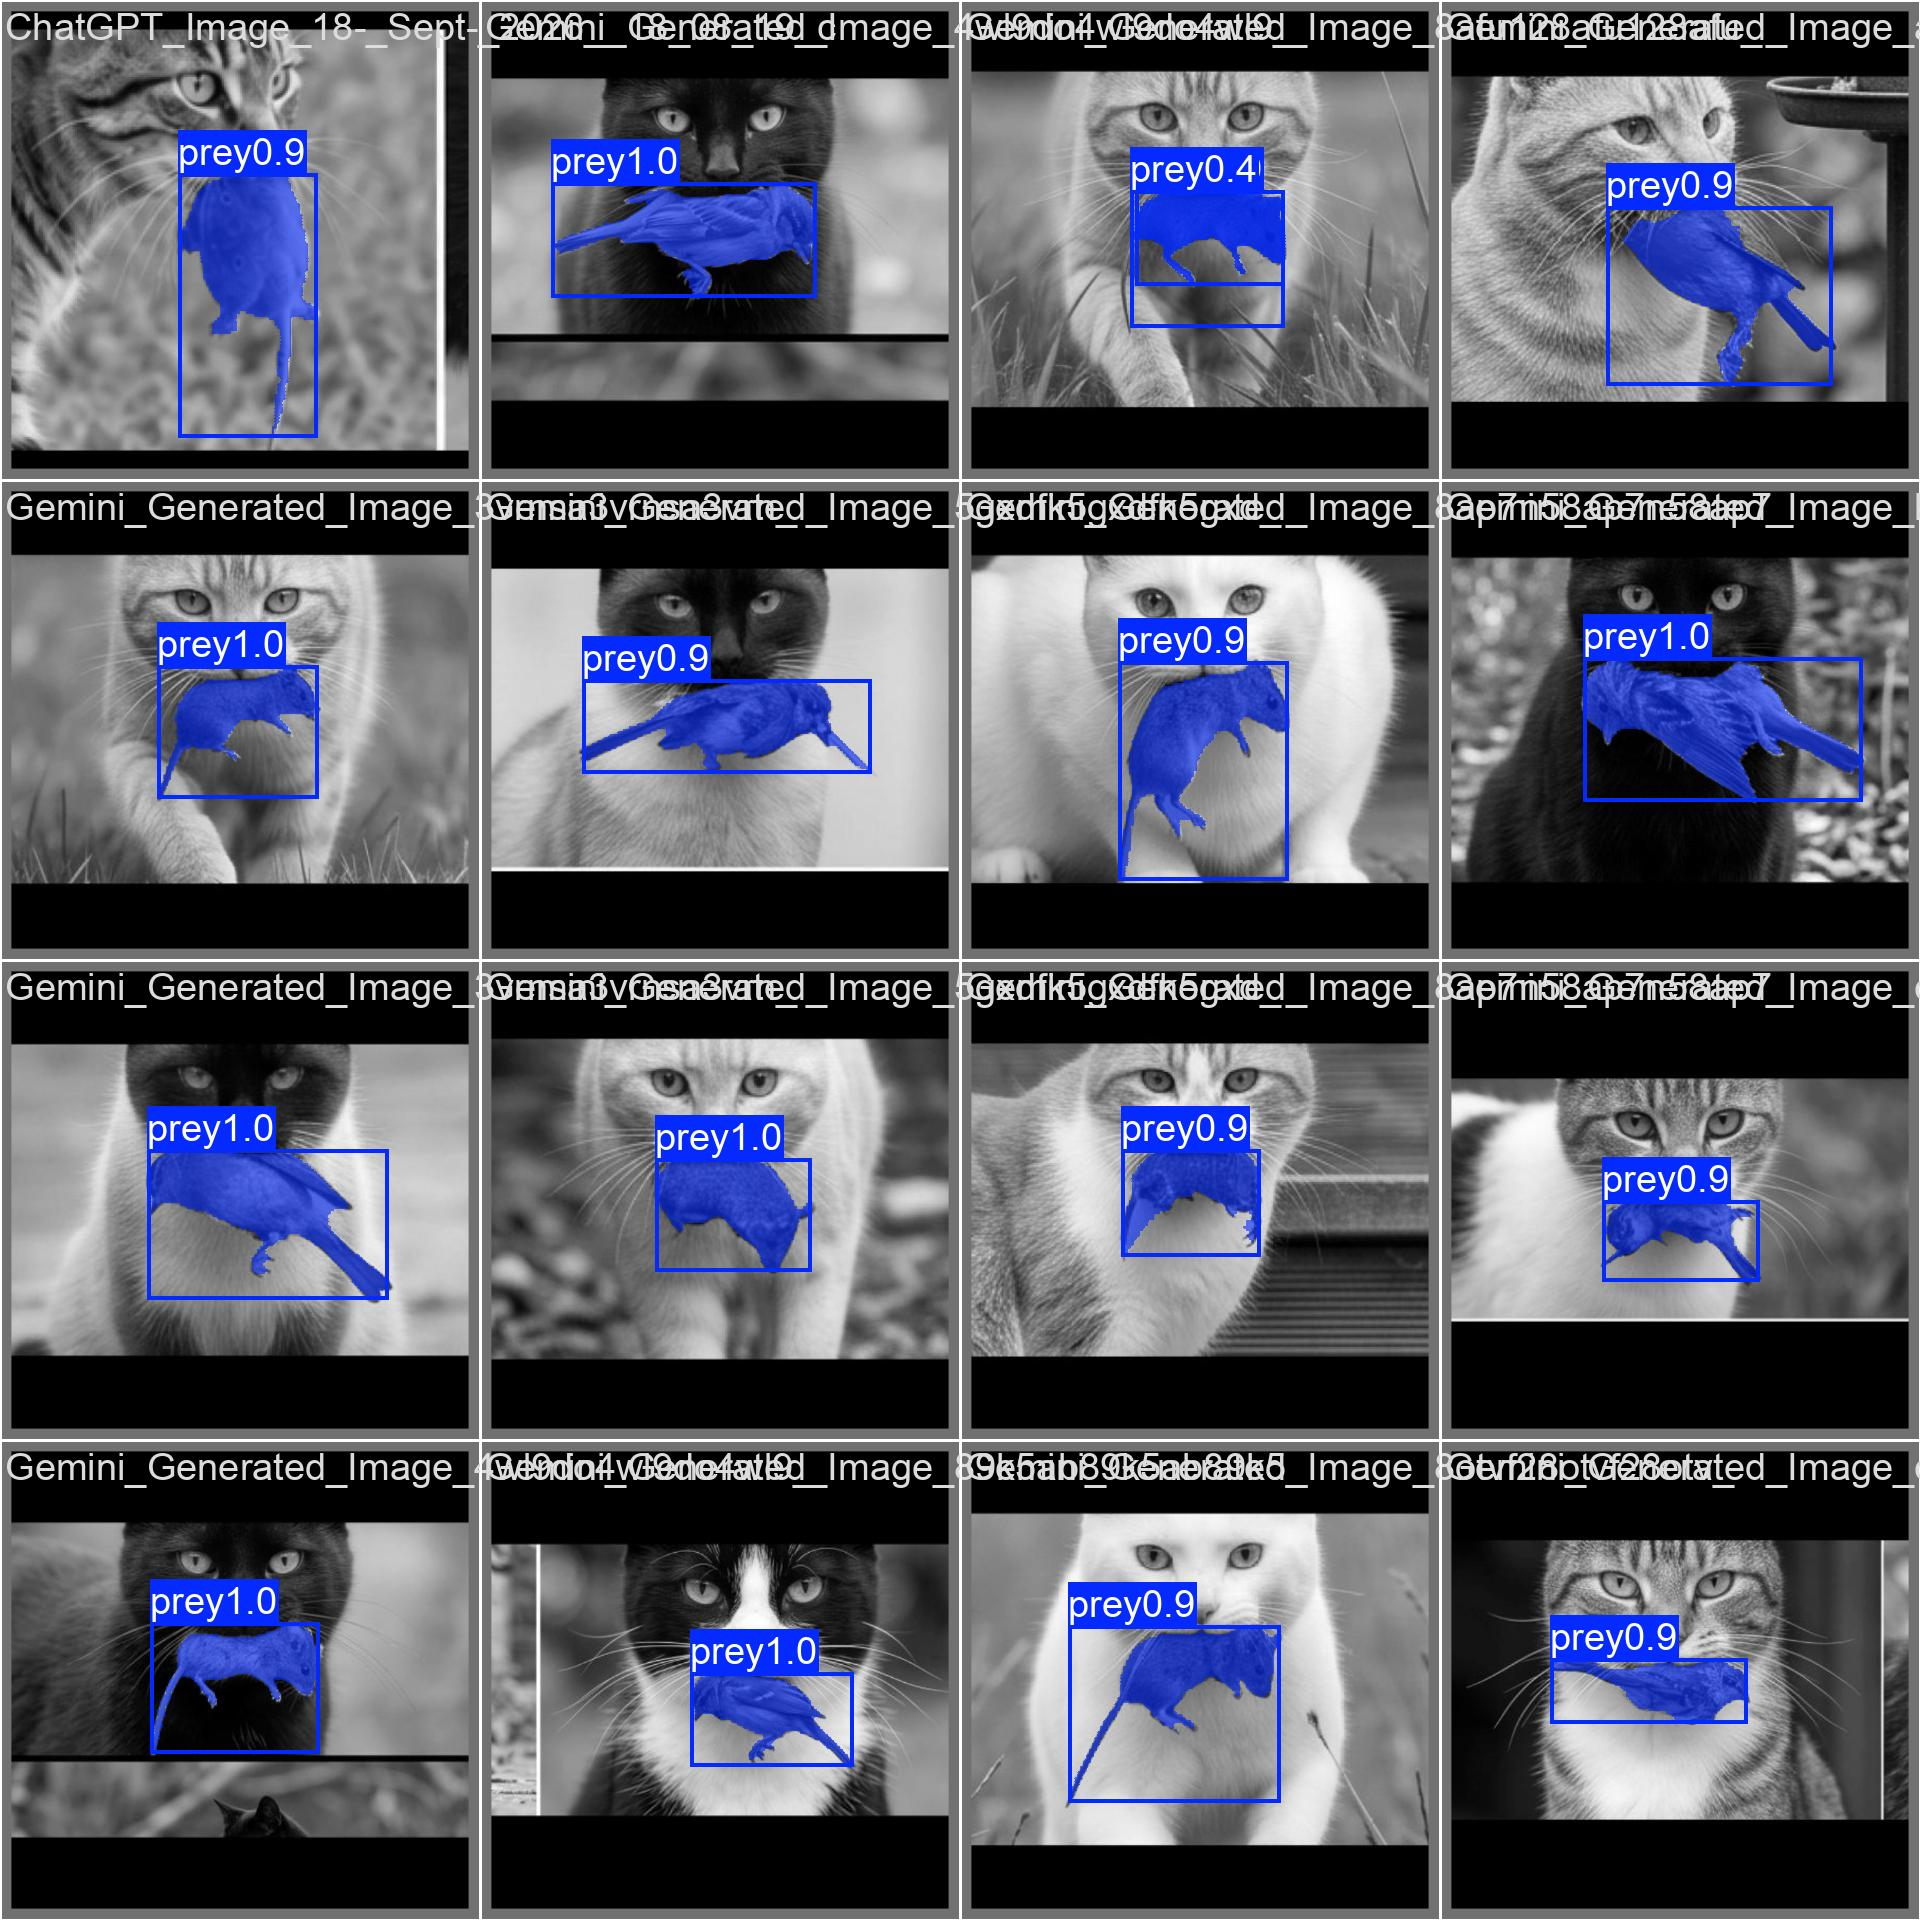
\includegraphics[width=0.8\textwidth]{images/seg_val_pred.jpg}
    \caption{Example predictions of the segmentation model on the validation dataset.}
    \label{fig:val_pred_cls}
\end{figure}

On paper alone, these models would make almost error-free predictions. The decisive question, however, is how the system behaves in practical use and which advantages the pipeline offers over pure detection and segmentation.

\section{Evaluation Methodology and Dataset}
\label{sec:evaluationsmethodik}
For the evaluation of the overall system, a dedicated test dataset of AI-generated video sequences is created. This section describes the structure of the dataset, the annotation of the reference data and the metrics used.

\subsection{Test Dataset}
The test basis consists of ten video pairs generated with the video model Veo via Gemini \cite{geminiteam2023gemini}. Each video shows the perspective of a fixed camera mounted directly above the cat flap, towards which one or two cats are moving. A video pair consists of a sequence in which a cat carries a prey animal in its mouth, and a counterpart with an identical scene and, as far as possible, an identical movement sequence, in which no cat carries prey. The two videos of a pair therefore differ solely in the presence of the prey.

The video pairs cover different fur colours, prey animals (mouse, bird, rat and vole), lighting conditions (day, dusk and infrared night vision) as well as scenes with two cats. The videos have a length of ten seconds at 24 frames per second. Since the system on the Raspberry Pi 5 processes around 8 frames per second, the videos are thinned out to 8 frames per second for the evaluation. As a result, the measured decision times correspond to real operation.

\subsection{Annotation of the Reference Data}
A reference annotation is created for each video. For each cat, it specifies the time intervals in which the cat is visible in the image, in which its face is recognisable and in which it is carrying prey. From these intervals, the correct state of the cat flap results for each frame: if at least one cat with prey is in the image, the flap must be locked; otherwise it may be opened.

\subsection{Definition of the System Metrics}
After all video sequences have passed through the pipeline, the metrics for the entire system can be computed. These are derived from the confusion matrix:

\begin{itemize}
    \item \textbf{True Positive (TP):} A cat with prey is not allowed into the house (correct locking).
    \item \textbf{False Negative (FN):} A cat with prey is allowed into the house (prey wrongly gets in).
    \item \textbf{True Negative (TN):} A cat without prey is allowed into the house (correct passage).
    \item \textbf{False Positive (FP):} A cat without prey is not allowed into the house (false alarm).
\end{itemize}

In the context of a cat flap, the cat has the highest priority from the user's point of view. A false positive (false alarm) means that the pet stands in front of a closed door for no reason. In order not to destroy the animal's trust in the flap, the evaluation focuses primarily on avoiding such false alarms (high precision). An occasional false negative (a mouse gets into the house) is deliberately accepted in exchange for stress-free use of the flap by the cat.


In contrast to an evaluation at video level, the frame-wise evaluation also captures brief wrong decisions. For each frame with a visible cat, the state of the flap is compared with the reference annotation. This yields the following indicators:

\begin{itemize}
    \item \emph{Safety error}: Proportion of frames in which the flap is open although a cat with prey is visible.
    \item \emph{Comfort error}: Proportion of frames in which the flap is locked although only clean cats are visible. Counting only starts after a decision time of three seconds from the detection of the cat face, since the state machine deliberately locks at the beginning.
    \item \emph{Precision}, \emph{recall} and \emph{F1 score} of the decision ``lock flap'' over all frames with a visible cat. Frames with clean cats within the decision time are not taken into account.
    \item \emph{Prey let through}: Number of videos with prey in which the flap was opened at least once.
    \item \emph{Decision time}: Time from the detection of the cat face until the first correct decision, i.e. until locking in the case of a cat with prey or until release in the case of a clean cat.
    \item \emph{Missed cats}: Proportion of frames with a recognisable cat face in which the system detects no cat.
\end{itemize}

The evaluation takes place in two steps. First, the detector and the segmentation model are run once per video and configuration, and the results of each frame are logged. Subsequently, the state machine is replicated on these logs. This makes it possible to compare different parameters of the state machine without repeating inference.

\section{Evaluation Results}
The overall system is evaluated in its final configuration: the face detector and the segmentation model work on greyscale images, and the state machine uses a time window of 20 frames and a threshold of 0.3. The derivation of these parameters is described in Section~\ref{sec:ablation_sm}. Table~\ref{tab:system_eval} summarises the results on the 20 videos of the test dataset.

\begin{table}[H]
    \centering
    \begin{tabular}{lcc}
        \toprule
        Metric & Videos with prey & Videos without prey \\
        \midrule
        Safety error & 1.0\,\% & -- \\
        Comfort error & -- & 3.3\,\% \\
        Prey let through & 2 of 10 & -- \\
        Clean cats locked out & -- & 0 of 10 \\
        Decision time & 0.13\,s & 0.60\,s \\
        \bottomrule
    \end{tabular}
    \caption{Results of the overall system on the test dataset.}
    \label{tab:system_eval}
\end{table}

Over all frames with a visible cat, the decision ``lock flap'' achieves a precision of 0.984, a recall of 0.990 and an F1 score of 0.987. In 4.3\,\% of the frames with a recognisable cat face, the system detects no cat. Broken down by lighting conditions, the safety error is 0.8\,\% for daytime recordings and 1.2\,\% for infrared recordings, and the comfort error is 5.6\,\% and 0.0\,\% respectively.

No clean cat is locked out permanently. In two of the ten videos with prey, the flap is briefly opened for four frames each (0.5~seconds). The analysis of these videos shows two causes:

\begin{itemize}
    \item At the beginning, the cat is still far from the camera, so the prey in the crop is too small to be detected by the segmentation model. If the average after 20 frames is still below the threshold, the cat is briefly released until the prey is detected.
    \item At the end of the video, the cat walks underneath the camera. The segmentation model returns no prey for these frames, and after the time window has elapsed, the cat is considered clean.
\end{itemize}

In the scenes with two cats, the tracker (ByteTrack) sometimes assigns the same cat a new identity several times. The resulting short-lived tracks do not block the release, since only cats that are visible in the current frame are taken into account. The release is thereby delayed in these scenes by up to 2.6~seconds, but remains within the decision time.

\section{Ablation Studies}
In the following ablation studies, one component of the system is removed or replaced in each case, while all other components remain unchanged. All studies use the test dataset and the metrics from Section~\ref{sec:evaluationsmethodik}.

\subsection{State Machine}
\label{sec:ablation_sm}
To validate the effectiveness and absolute necessity of the temporal aggregation (state machine), an ablation study was carried out. Note: An initial lock is intended: even if the cat is not carrying prey, it is denied access until it proves that it is clean. Comfort errors are therefore only counted after the decision time of three seconds. In this study, the exact same system was applied twice to all 20 test videos:

\begin{enumerate}
    \item \textbf{Full system:} With the state machine active and a moving average over 20 frames (\texttt{history\_length=20}).
    \item \textbf{Ablation:} Since the state machine was deactivated, the decision about locking the flap was based exclusively on the result of the current frame (\texttt{history\_length=1}).
\end{enumerate}


Table~\ref{tab:sm_ablation} compares both configurations. For the decision based on the current frame, a threshold of 0.5 is used; for the full system, the threshold of 0.3 from the subsequent parameter sweep.

\begin{table}[H]
    \centering
    \begin{tabular}{lrr}
        \toprule
        Metric & Without state machine & With state machine \\
        \midrule
        Safety error & 17.0\,\% & 1.0\,\% \\
        Comfort error & 19.7\,\% & 3.3\,\% \\
        Precision & 0.896 & 0.984 \\
        Recall & 0.830 & 0.990 \\
        F1 score & 0.862 & 0.987 \\
        Prey let through & 10 of 10 & 2 of 10 \\
        Clean cats locked out & 0 of 10 & 0 of 10 \\
        \bottomrule
    \end{tabular}
    \caption{Two-stage system without state machine (time window of one frame, threshold 0.5) and with state machine (time window of 20 frames, threshold 0.3).}
    \label{tab:sm_ablation}
\end{table}

Without the state machine, the flap is open in 17.0\,\% of the frames with prey, and in each of the ten videos with prey the flap is released at least once. At the same time, the flap is locked in 19.7\,\% of the frames with clean cats. Individual wrong decisions of the segmentation model directly affect the state of the flap without temporal aggregation. With the state machine, the safety error drops to 1.0\,\% and the comfort error to 3.3\,\%.

In addition, a parameter sweep over the length of the time window (1, 3, 5, 8, 10, 15 and 20 frames) and the threshold (0.3 to 0.8) is evaluated. It shows the trade-off between safety errors, comfort errors and decision time and serves to determine the final parameters. Table~\ref{tab:sm_sweep} contains the results of all combinations. The proportion of missed cats is 4.3\,\% in all combinations, since it depends only on the detector. In no combination is a clean cat locked out permanently.

\begin{table}[H]
    \centering
    \footnotesize
    \renewcommand{\arraystretch}{0.92}
    \begin{tabular}{rrrrrrrr}
        \toprule
        & & & & & Prey let & \multicolumn{2}{c}{Decision time [s]} \\
        \cmidrule(lr){7-8}
        Window & Threshold & Safety err. & Comfort err. & F1 & through & Prey & clean \\
        \midrule
        1 & 0.3 & 11.6\,\% & 19.2\,\% & 0.894 & 9/10 & 0.03 & 0.00 \\
        1 & 0.4 & 12.5\,\% & 19.2\,\% & 0.889 & 10/10 & 0.03 & 0.00 \\
        1 & 0.5 & 17.0\,\% & 19.7\,\% & 0.862 & 10/10 & 0.46 & 0.00 \\
        1 & 0.6 & 17.2\,\% & 20.3\,\% & 0.859 & 10/10 & 0.46 & 0.00 \\
        1 & 0.7 & 18.5\,\% & 20.3\,\% & 0.852 & 10/10 & 0.46 & 0.00 \\
        1 & 0.8 & 23.8\,\% & 20.3\,\% & 0.819 & 10/10 & 0.58 & 0.00 \\
        \midrule
        3 & 0.3 & 10.5\,\% & 20.0\,\% & 0.898 & 9/10 & 0.03 & 0.00 \\
        3 & 0.4 & 11.2\,\% & 20.3\,\% & 0.894 & 9/10 & 0.03 & 0.00 \\
        3 & 0.5 & 16.2\,\% & 20.5\,\% & 0.865 & 9/10 & 0.46 & 0.00 \\
        3 & 0.6 & 20.2\,\% & 12.3\,\% & 0.859 & 10/10 & 0.46 & 0.00 \\
        3 & 0.7 & 25.8\,\% & 10.5\,\% & 0.828 & 10/10 & 0.46 & 0.00 \\
        3 & 0.8 & 31.1\,\% & 10.5\,\% & 0.792 & 10/10 & 0.06 & 0.00 \\
        \midrule
        5 & 0.3 & 7.1\,\% & 20.8\,\% & 0.915 & 9/10 & 0.03 & 0.00 \\
        5 & 0.4 & 7.8\,\% & 20.5\,\% & 0.912 & 9/10 & 0.03 & 0.00 \\
        5 & 0.5 & 21.2\,\% & 10.5\,\% & 0.857 & 9/10 & 0.51 & 0.00 \\
        5 & 0.6 & 24.1\,\% & 3.3\,\% & 0.855 & 10/10 & 0.54 & 0.00 \\
        5 & 0.7 & 25.6\,\% & 3.3\,\% & 0.845 & 10/10 & 0.61 & 0.00 \\
        5 & 0.8 & 30.8\,\% & 3.3\,\% & 0.811 & 10/10 & 0.43 & 0.00 \\
        \midrule
        8 & 0.3 & 5.4\,\% & 18.7\,\% & 0.929 & 8/10 & 0.04 & 0.11 \\
        8 & 0.4 & 9.6\,\% & 12.6\,\% & 0.920 & 9/10 & 0.05 & 0.11 \\
        8 & 0.5 & 16.4\,\% & 3.3\,\% & 0.903 & 9/10 & 0.55 & 0.11 \\
        8 & 0.6 & 19.5\,\% & 3.3\,\% & 0.884 & 9/10 & 0.57 & 0.11 \\
        8 & 0.7 & 23.1\,\% & 3.3\,\% & 0.861 & 10/10 & 0.65 & 0.11 \\
        8 & 0.8 & 33.6\,\% & 3.3\,\% & 0.790 & 10/10 & 0.36 & 0.11 \\
        \midrule
        10 & 0.3 & 4.0\,\% & 12.6\,\% & 0.950 & 6/10 & 0.05 & 0.14 \\
        10 & 0.4 & 5.9\,\% & 3.3\,\% & 0.962 & 8/10 & 0.06 & 0.14 \\
        10 & 0.5 & 11.9\,\% & 3.3\,\% & 0.929 & 9/10 & 0.54 & 0.14 \\
        10 & 0.6 & 16.4\,\% & 3.3\,\% & 0.903 & 9/10 & 0.64 & 0.14 \\
        10 & 0.7 & 19.1\,\% & 3.3\,\% & 0.886 & 9/10 & 0.73 & 0.14 \\
        10 & 0.8 & 36.2\,\% & 3.3\,\% & 0.771 & 10/10 & 0.39 & 0.14 \\
        \midrule
        15 & 0.3 & 1.8\,\% & 3.3\,\% & 0.983 & 4/10 & 0.08 & 0.20 \\
        15 & 0.4 & 4.1\,\% & 3.3\,\% & 0.971 & 5/10 & 0.16 & 0.20 \\
        15 & 0.5 & 11.4\,\% & 3.3\,\% & 0.932 & 6/10 & 0.66 & 0.20 \\
        15 & 0.6 & 13.1\,\% & 3.3\,\% & 0.922 & 8/10 & 0.79 & 0.20 \\
        15 & 0.7 & 14.9\,\% & 3.3\,\% & 0.912 & 9/10 & 0.96 & 0.20 \\
        15 & 0.8 & 28.7\,\% & 3.3\,\% & 0.824 & 10/10 & 0.67 & 0.20 \\
        \midrule
        \textbf{20} & \textbf{0.3} & \textbf{1.0\,\%} & \textbf{3.3\,\%} & \textbf{0.987} & \textbf{2/10} & \textbf{0.13} & \textbf{0.60} \\
        20 & 0.4 & 1.8\,\% & 3.3\,\% & 0.983 & 3/10 & 0.21 & 0.60 \\
        20 & 0.5 & 6.9\,\% & 3.3\,\% & 0.956 & 6/10 & 0.78 & 0.60 \\
        20 & 0.6 & 8.4\,\% & 3.3\,\% & 0.948 & 6/10 & 1.00 & 0.60 \\
        20 & 0.7 & 11.0\,\% & 3.3\,\% & 0.934 & 9/10 & 1.31 & 0.60 \\
        20 & 0.8 & 24.4\,\% & 3.3\,\% & 0.853 & 10/10 & 1.19 & 0.60 \\
        \bottomrule
    \end{tabular}
    \caption{Parameter sweep of the state machine over the length of the time window (in frames) and the threshold. The selected configuration is highlighted in bold. A time window of one frame corresponds to a system without a state machine.}
    \label{tab:sm_sweep}
\end{table}

The following relationships can be read from the parameter sweep:

\begin{itemize}
    \item \emph{Length of the time window}: At a threshold of 0.3, both the safety error (from 11.6\,\% to 1.0\,\%) and the number of videos in which prey is let through (from 9 to 2) decrease as the time window grows longer. Brief wrong decisions of the segmentation model are averaged over more frames and less often lead to a release. This relationship cannot be observed at high thresholds. From a time window of ten frames onwards, the comfort error remains constant at 3.3\,\% for thresholds of 0.4 and above.
    \item \emph{Threshold}: A low threshold locks the flap even at a small average proportion of prey. This reduces the safety error, but for time windows of three to ten frames the comfort error increases. For long time windows, the comfort error remains at 3.3\,\% even at a threshold of 0.3.
    \item \emph{Decision time}: Longer time windows delay the release for clean cats, since the state machine first has to collect a sufficient history. At the same time, the time until locking for cats with prey generally increases with the threshold. At 20 frames, the mean decision time for clean cats is 0.60~seconds and is thus clearly below the decision time of three seconds.
\end{itemize}

The combination of a time window of 20 frames and a threshold of 0.3 achieves the lowest safety error (1.0\,\%), the highest F1 score (0.987) and the lowest number of videos with prey let through (2 of 10). The comfort error of 3.3\,\% is the lowest value of the entire parameter sweep, and no clean cat is locked out. At 8 frames per second, the time window corresponds to a history of 2.5~seconds. This configuration is therefore set as the final parametrisation of the state machine and used in all following ablation studies.

\subsection{Detection and Segmentation versus Detection}
\label{sec:ablation_1stage}
To validate the architecture of our two-stage chain (detector + segmentation model), a single-stage object detector (YOLO26) was trained for this study. It has two classes: ``cat with prey'' and ``cat without prey''. Both classes contain the same amount of data.

\begin{figure}[H]
    \centering
    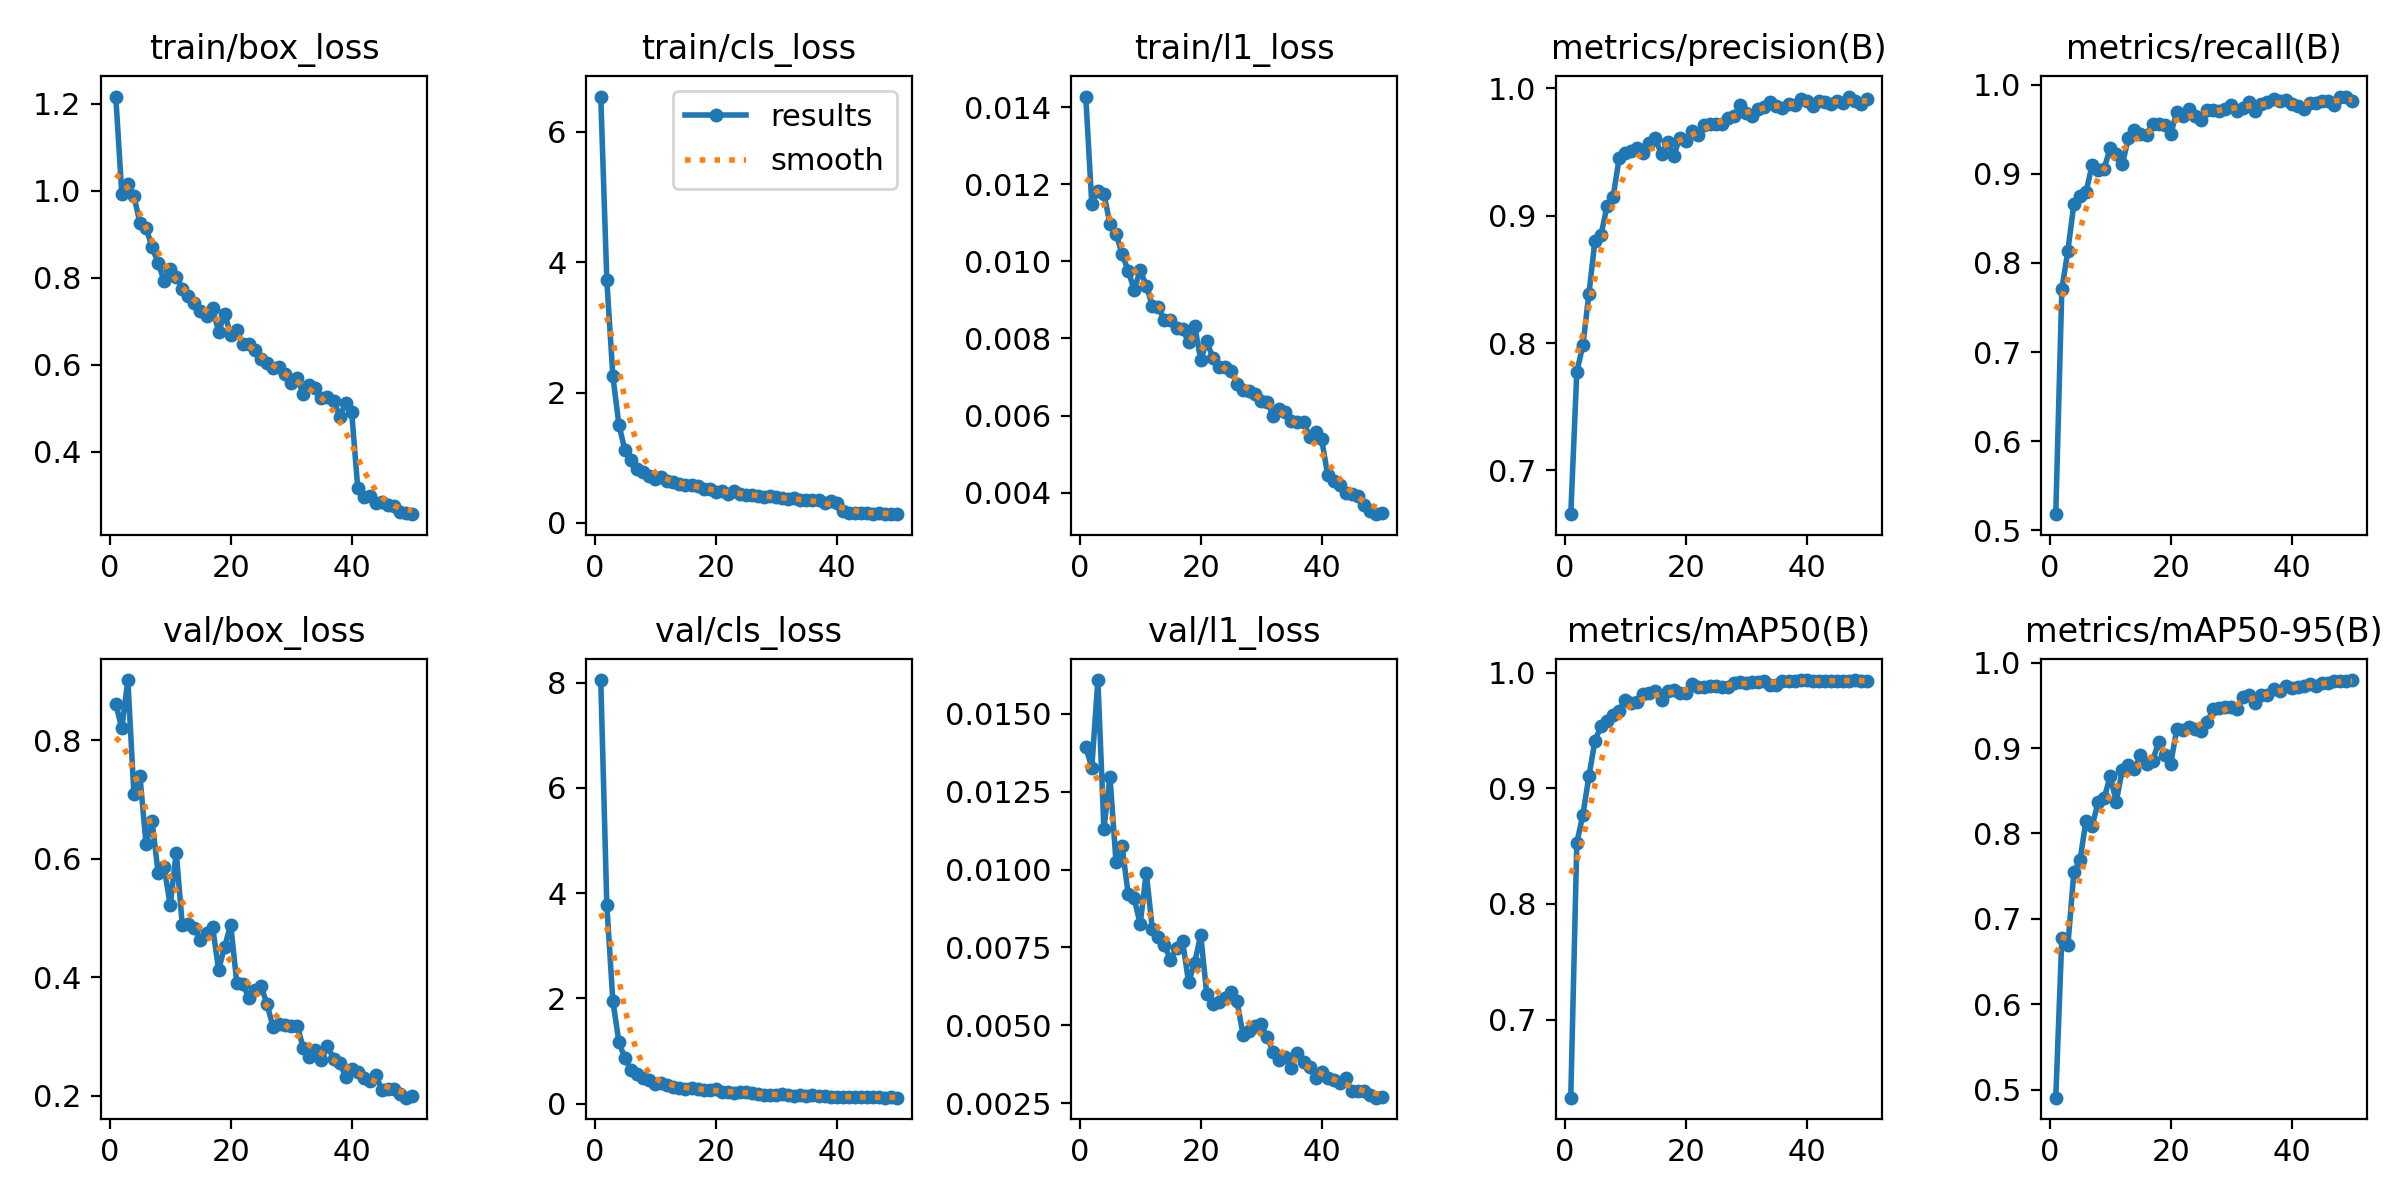
\includegraphics[width=0.8\textwidth]{images/1stage_ablation_results.png}
    \caption{Training metrics of the single-stage object detector.}
    \label{fig:ablation_1stage_train}
\end{figure}

\begin{figure}[H]
    \centering
    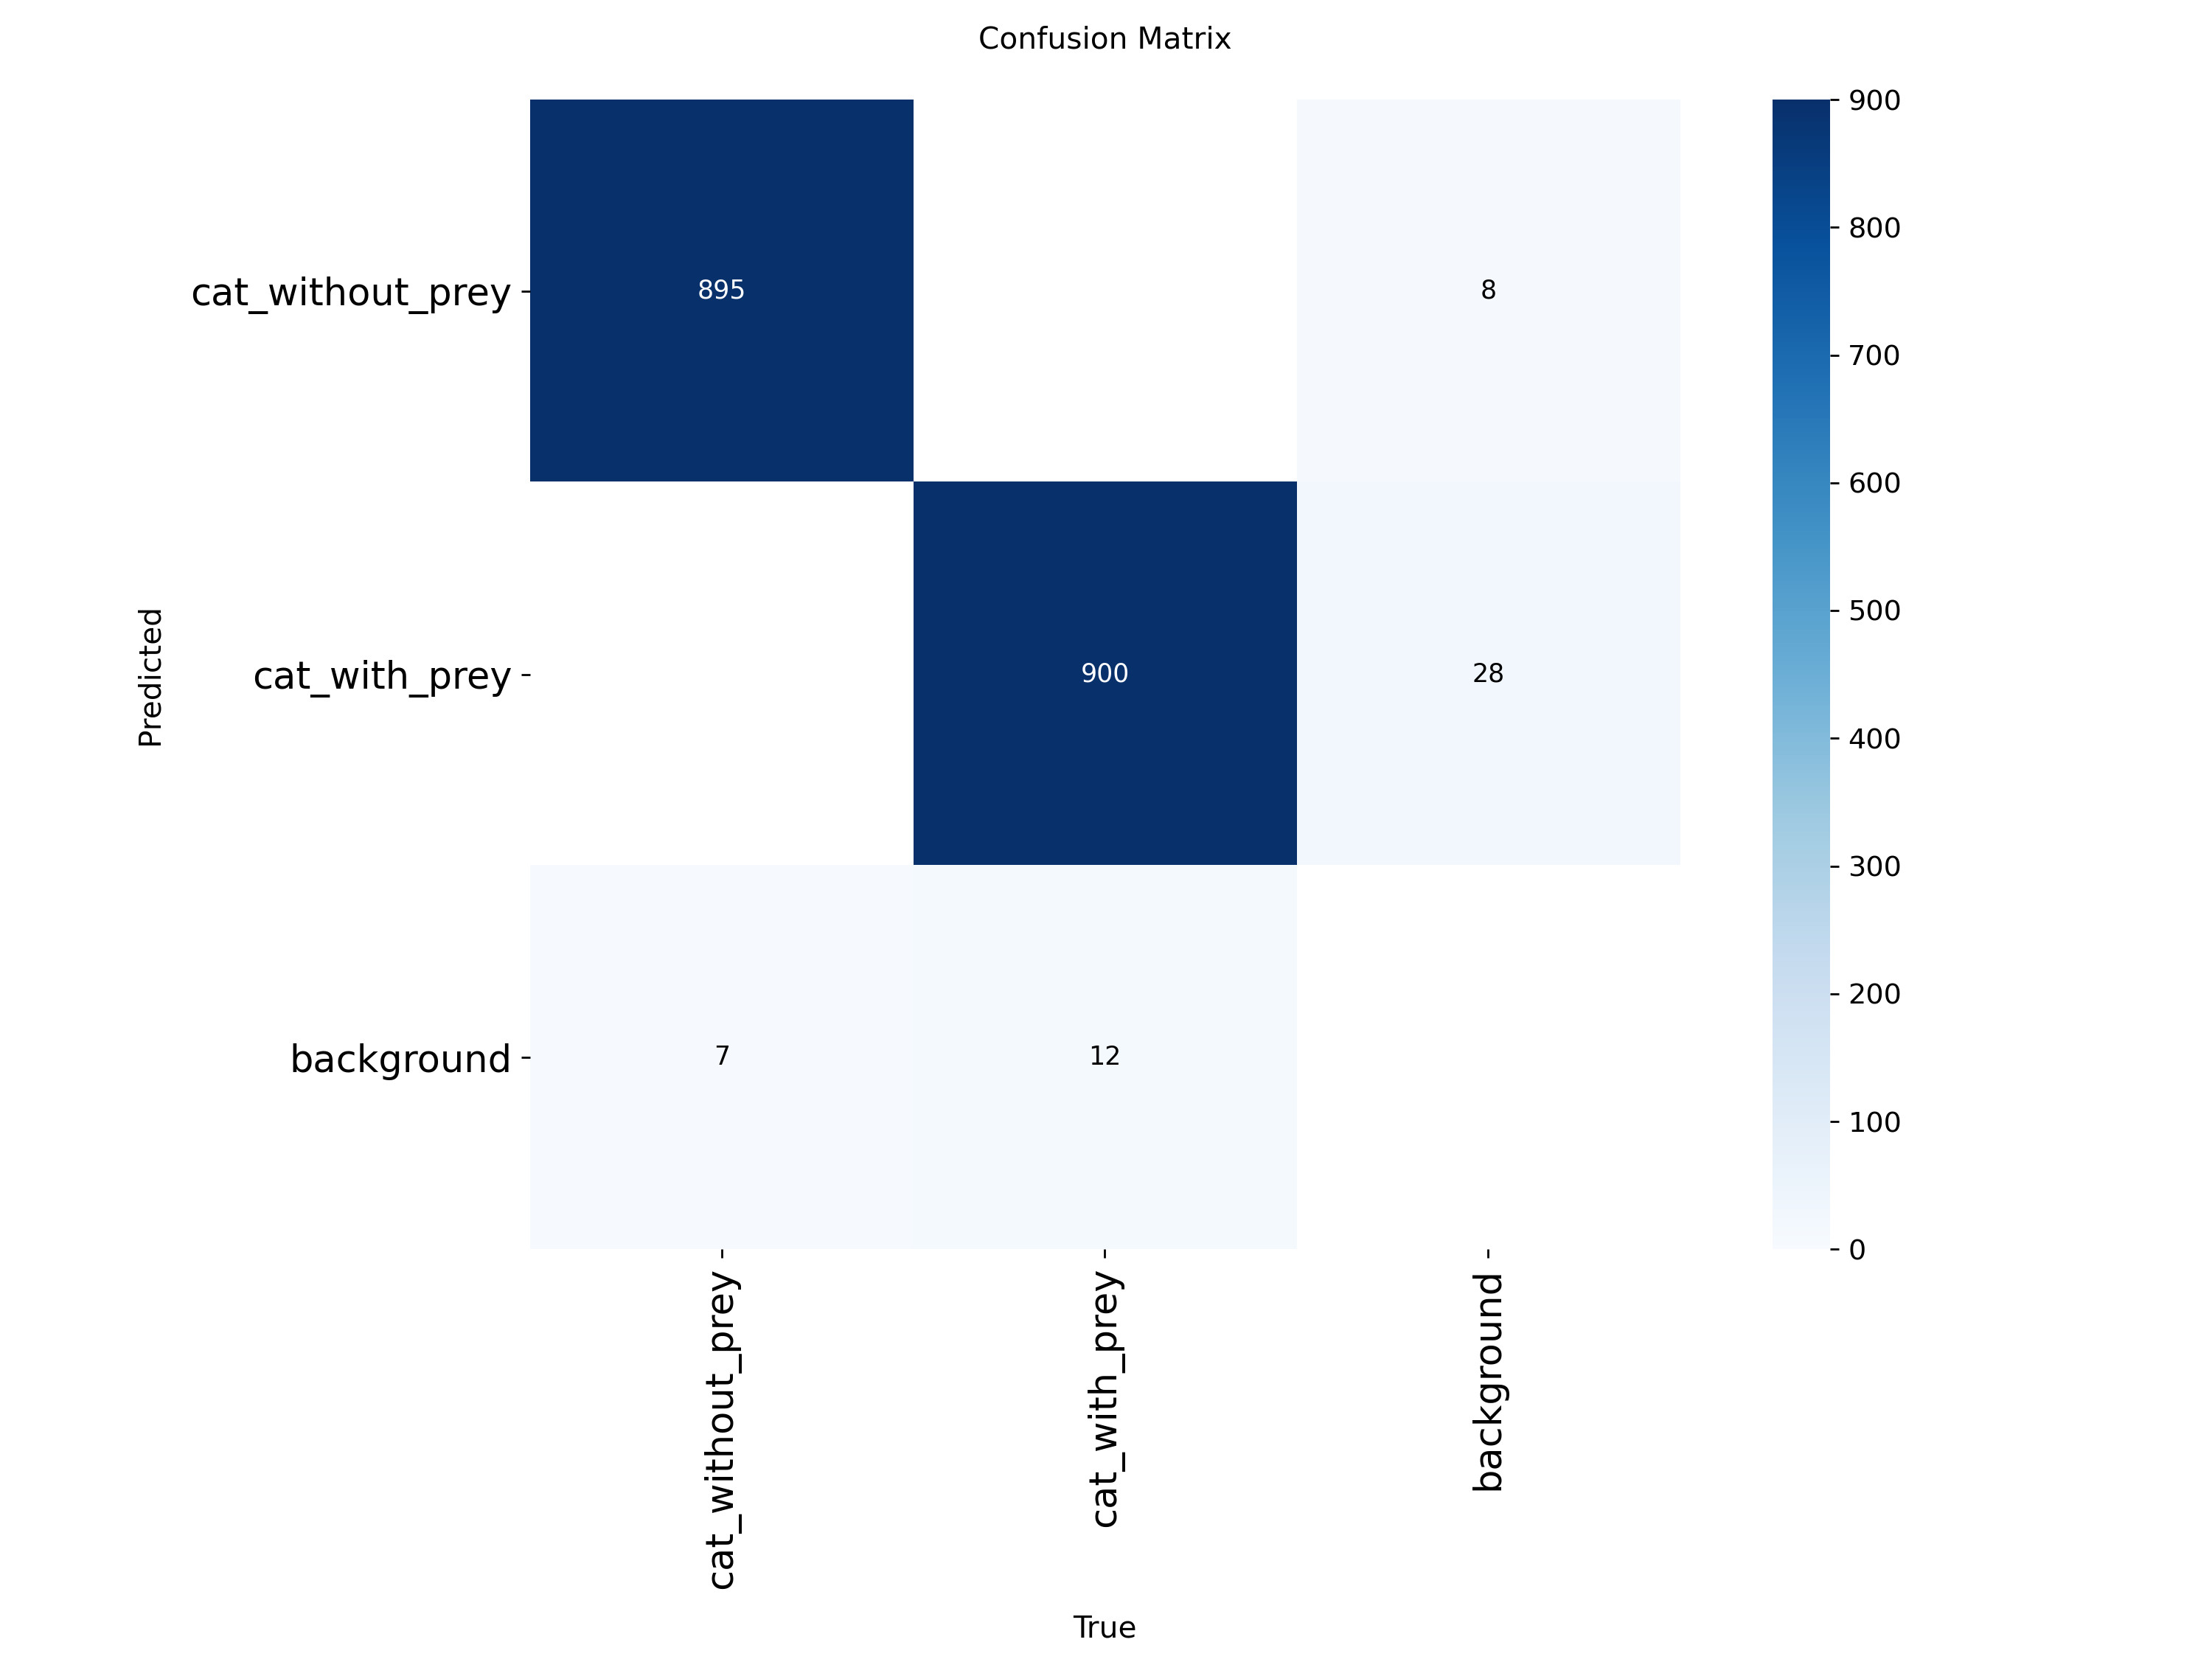
\includegraphics[width=0.7\textwidth]{images/1stage_ablation_confusionmatrix.png}
    \caption{Confusion matrix of the single-stage object detector on the validation data.}
    \label{fig:ablation_1stage_conf}
\end{figure}


To compare the models in isolation, the state machine was deactivated again (\texttt{history\_length=1}). We evaluated how many safety and comfort errors both systems made, as well as how many cats were missed in the video overall.
In addition, both systems are evaluated with the state machine in the final configuration (time window of 20 frames, threshold 0.3). Table~\ref{tab:ablation_1stage} shows the results of both variants.

\begin{table}[H]
    \centering
    \begin{tabular}{lrrrr}
        \toprule
        & \multicolumn{2}{c}{Without state machine} & \multicolumn{2}{c}{With state machine} \\
        \cmidrule(lr){2-3}\cmidrule(lr){4-5}
        Metric & Two-stage & Single-stage & Two-stage & Single-stage \\
        \midrule
        Safety error & 17.0\,\% & 9.9\,\% & 1.0\,\% & 10.6\,\% \\
        Comfort error & 19.7\,\% & 61.5\,\% & 3.3\,\% & 29.7\,\% \\
        Precision & 0.896 & 0.750 & 0.984 & 0.860 \\
        Recall & 0.830 & 0.901 & 0.990 & 0.894 \\
        F1 score & 0.862 & 0.819 & 0.987 & 0.877 \\
        Missed cats & 4.3\,\% & 6.5\,\% & 4.3\,\% & 6.5\,\% \\
        Prey let through & 10 of 10 & 8 of 10 & 2 of 10 & 2 of 10 \\
        Decision time (clean) & 0.00\,s & 2.54\,s & 0.60\,s & 3.02\,s \\
        \bottomrule
    \end{tabular}
    \caption{Comparison of the two-stage system (detection and segmentation) with the single-stage object detector, without state machine (time window of one frame, threshold 0.5) and with state machine (time window of 20 frames, threshold 0.3).}
    \label{tab:ablation_1stage}
\end{table}

At 6.5\,\%, the single-stage system misses more cats than the face detector of the two-stage system (4.3\,\%). The clearest difference is in the comfort error: without the state machine, the flap is locked in 61.5\,\% of the frames with clean cats, and with the state machine in 29.7\,\%. The single-stage detector frequently assigns clean cats to the class ``cat with prey''. As a result, without the state machine it achieves a lower safety error than the two-stage system, but this comes at the expense of the clean cats. With the state machine, both systems let prey through in two of ten videos. However, the safety error of the single-stage system, at 10.6\,\%, is around ten times as high as that of the two-stage system (1.0\,\%). The F1 score of the two-stage system, at 0.987, is clearly above that of the single-stage system (0.877). In addition, the single-stage system needs 3.02~seconds on average until a clean cat is released and thus exceeds the decision time of three seconds.

\subsection{Greyscale versus Colour Images}
Since the camera switches to infrared night vision in darkness, the system works on greyscale images throughout. In this study, a system trained on greyscale images is compared with a system trained on colour images, broken down by daytime and night-time recordings.
Both segmentation models have the same architecture (YOLO26n-seg) and are trained with the same training data. The colour model receives the original colour images, the greyscale model the images converted to greyscale. The face detector and the state machine (time window of 20 frames, threshold 0.3) remain unchanged in both configurations. The daytime recordings comprise six video pairs, the infrared recordings four. Table~\ref{tab:ablation_gray} shows the results.

\begin{table}[H]
    \centering
    \small
    \begin{tabular}{lrrrrrr}
        \toprule
        & \multicolumn{2}{c}{Day} & \multicolumn{2}{c}{Infrared} & \multicolumn{2}{c}{Overall} \\
        \cmidrule(lr){2-3}\cmidrule(lr){4-5}\cmidrule(lr){6-7}
        Metric & Grey & Colour & Grey & Colour & Grey & Colour \\
        \midrule
        Safety error & 0.8\,\% & 4.4\,\% & 1.2\,\% & 5.6\,\% & 1.0\,\% & 4.9\,\% \\
        Comfort error & 5.6\,\% & 0.0\,\% & 0.0\,\% & 0.0\,\% & 3.3\,\% & 0.0\,\% \\
        Precision & 0.973 & 1.000 & 1.000 & 1.000 & 0.984 & 1.000 \\
        Recall & 0.992 & 0.956 & 0.988 & 0.944 & 0.990 & 0.951 \\
        F1 score & 0.982 & 0.978 & 0.994 & 0.971 & 0.987 & 0.975 \\
        Prey let through & 1 of 6 & 2 of 6 & 1 of 4 & 2 of 4 & 2 of 10 & 4 of 10 \\
        Decision time (prey) & 0.19\,s & 0.94\,s & 0.03\,s & 0.75\,s & 0.13\,s & 0.86\,s \\
        \bottomrule
    \end{tabular}
    \caption{Comparison of the segmentation model for greyscale images with the segmentation model for colour images, broken down by daytime and infrared recordings.}
    \label{tab:ablation_gray}
\end{table}

For daytime recordings, both models achieve a similar F1 score (0.982 versus 0.978). The greyscale model has a lower safety error (0.8\,\% versus 4.4\,\%), the colour model a lower comfort error (0.0\,\% versus 5.6\,\%). For infrared recordings, no colour information is available. Here the greyscale model achieves a clearly lower safety error (1.2\,\% versus 5.6\,\%) and a higher F1 score (0.994 versus 0.971), while neither model shows a comfort error. In addition, the greyscale model locks the flap for cats with prey after 0.13~seconds on average, the colour model only after 0.86~seconds. Over the entire test dataset, the greyscale model achieves the higher F1 score and lets prey through in two instead of four videos.
